%%%%%%%%%%%%%%%%%%%%%%%%%%%%%%%%%%%%%%%%%
% Masters/Doctoral Thesis 
% LaTeX Template
% Version 2.4 (22/11/16)
%
% This template has been downloaded from:
% http://www.LaTeXTemplates.com
%
% Version 2.x major modifications by:
% Vel (vel@latextemplates.com)
%
% This template is based on a template by:
% Steve Gunn (http://users.ecs.soton.ac.uk/srg/softwaretools/document/templates/)
% Sunil Patel (http://www.sunilpatel.co.uk/thesis-template/)
%
% Template license:
% CC BY-NC-SA 3.0 (http://creativecommons.org/licenses/by-nc-sa/3.0/)
%
%%%%%%%%%%%%%%%%%%%%%%%%%%%%%%%%%%%%%%%%%

%----------------------------------------------------------------------------------------
%	PACKAGES AND OTHER DOCUMENT CONFIGURATIONS
%----------------------------------------------------------------------------------------

\documentclass[
11pt, % The default document font size, options: 10pt, 11pt, 12pt
%oneside, % Two side (alternating margins) for binding by default, uncomment to switch to one side
english, % ngerman for German
singlespacing, % Single line spacing, alternatives: onehalfspacing or doublespacing
%draft, % Uncomment to enable draft mode (no pictures, no links, overfull hboxes indicated)
%nolistspacing, % If the document is onehalfspacing or doublespacing, uncomment this to set spacing in lists to single
%liststotoc, % Uncomment to add the list of figures/tables/etc to the table of contents
%toctotoc, % Uncomment to add the main table of contents to the table of contents
%parskip, % Uncomment to add space between paragraphs
%nohyperref, % Uncomment to not load the hyperref package
headsepline, % Uncomment to get a line under the header
%chapterinoneline, % Uncomment to place the chapter title next to the number on one line
%consistentlayout, % Uncomment to change the layout of the declaration, abstract and acknowledgements pages to match the default layout
]{MastersDoctoralThesis} % The class file specifying the document structure
\usepackage{listings}
\lstset{language=Haskell}
\usepackage[utf8]{inputenc} % Required for inputting international characters
\usepackage[T1]{fontenc} % Output font encoding for international characters

\usepackage{palatino} % Use the Palatino font by default

\usepackage[backend=biber,style=authoryear,natbib=true]{biblatex} % Use the bibtex backend with the authoryear citation style (which resembles APA)

\addbibresource{example.bib} % The filename of the bibliography

\usepackage[autostyle=true]{csquotes} % Required to generate language-dependent quotes in the bibliography

%----------------------------------------------------------------------------------------
%	MARGIN SETTINGS
%----------------------------------------------------------------------------------------

\geometry{
	paper=a4paper, % Change to letterpaper for US letter
	inner=2.5cm, % Inner margin
	outer=3.8cm, % Outer margin
	bindingoffset=.5cm, % Binding offset
	top=1.5cm, % Top margin
	bottom=1.5cm, % Bottom margin
	%showframe, % Uncomment to show how the type block is set on the page
}

%----------------------------------------------------------------------------------------
%	THESIS INFORMATION
%----------------------------------------------------------------------------------------

\thesistitle{Alternative Software Transaction Implementation in Haskell} % Your thesis title, this is used in the title and abstract, print it elsewhere with \ttitle
\supervisor{Dr. Frank Huch} % Your supervisor's name, this is used in the title page, print it elsewhere with \supname
\examiner{} % Your examiner's name, this is not currently used anywhere in the template, print it elsewhere with \examname
\degree{Master of Science} % Your degree name, this is used in the title page and abstract, print it elsewhere with \degreename
\author{Lasse Folger} % Your name, this is used in the title page and abstract, print it elsewhere with \authorname
\addresses{} % Your address, this is not currently used anywhere in the template, print it elsewhere with \addressname

\subject{Concurrent Programming} % Your subject area, this is not currently used anywhere in the template, print it elsewhere with \subjectname
\keywords{Software Transactions, Haskell, Synchronization, Concurrent Programming} % Keywords for your thesis, this is not currently used anywhere in the template, print it elsewhere with \keywordnames
\university{\href{http://www.uni-kiel.de}{Christian-Albrechts-University}} % Your university's name and URL, this is used in the title page and abstract, print it elsewhere with \univname
\department{\href{https://www.inf.uni-kiel.de/en}{Department of Computer Science}} % Your department's name and URL, this is used in the title page and abstract, print it elsewhere with \deptname
\group{\href{http://www.ps.informatik.uni-kiel.de/en/welcome-to-the-home-of-the-research-group?set_language=en}{Programming Languages and Compiler Construction}} % Your research group's name and URL, this is used in the title page, print it elsewhere with \groupname
\faculty{\href{http://www.tf.uni-kiel.de/en}{Faculty of Engineering}} % Your faculty's name and URL, this is used in the title page and abstract, print it elsewhere with \facname

\AtBeginDocument{
\hypersetup{pdftitle={Alternative Software Transaction Implementation in Haskell}} % Set the PDF's title to your title
\hypersetup{pdfauthor={Lasse Folger}} % Set the PDF's author to your name
\hypersetup{pdfkeywords={Software Transactions, Haskell}} % Set the PDF's keywords to your keywords
\hypersetup{urlcolor=blue}
\hypersetup{colorlinks=false}
}

\begin{document}

\frontmatter % Use roman page numbering style (i, ii, iii, iv...) for the pre-content pages

\pagestyle{plain} % Default to the plain heading style until the thesis style is called for the body content

%----------------------------------------------------------------------------------------
%	TITLE PAGE
%----------------------------------------------------------------------------------------

\begin{titlepage}
\begin{center}

\vspace*{.06\textheight}
{\scshape\LARGE \univname\par}\vspace{1.5cm} % University name
\textsc{\Large Master Thesis}\\[0.5cm] % Thesis type

\HRule \\[0.4cm] % Horizontal line
{\huge \bfseries \ttitle\par}\vspace{0.4cm} % Thesis title
\HRule \\[1.5cm] % Horizontal line
 
\begin{minipage}[t]{0.4\textwidth}
\begin{flushleft} \large
\emph{Author:}\\
\authorname % Author name - remove the \href bracket to remove the link
\end{flushleft}
\end{minipage}
\begin{minipage}[t]{0.4\textwidth}
\begin{flushright} \large
\emph{Supervisor:} \\
\supname % Supervisor name - remove the \href bracket to remove the link  
\end{flushright}
\end{minipage}\\[3cm]
 
\vfill

\large \textit{A thesis submitted in fulfillment of the requirements\\ for the degree of \degreename}\\[0.3cm] % University requirement text
\textit{in the}\\[0.4cm]
\groupname\\\deptname\\[2cm] % Research group name and department name
 
\vfill

{\large \today}\\[4cm] % Date
%\includegraphics{Logo} % University/department logo - uncomment to place it
 
\vfill
\end{center}
\end{titlepage}

%----------------------------------------------------------------------------------------
%	DECLARATION PAGE
%----------------------------------------------------------------------------------------

\begin{declaration}
\addchaptertocentry{\authorshipname} % Add the declaration to the table of contents
\bigskip\noindent Hiermit erkl{\"a}re ich an Eides statt, dass
ich die vorliegende Arbeit selbst\-st{\"a}n\-dig verfasst und keine
anderen als die angegebenen Quellen und Hilfsmittel verwendet habe.\par
\bigskip\noindent Kiel, \today
\vskip 10mm
\hfill\rule{18em}{.3pt}%
% 
% 
% 
% 
% \noindent I, \authorname, declare that this thesis titled, \enquote{\ttitle} and the work presented in it are my own. I confirm that:
% 
% \begin{itemize} 
% \item This work was done wholly or mainly while in candidature for a research degree at this University.
% \item Where any part of this thesis has previously been submitted for a degree or any other qualification at this University or any other institution, this has been clearly stated.
% \item Where I have consulted the published work of others, this is always clearly attributed.
% \item Where I have quoted from the work of others, the source is always given. With the exception of such quotations, this thesis is entirely my own work.
% \item I have acknowledged all main sources of help.
% \item Where the thesis is based on work done by myself jointly with others, I have made clear exactly what was done by others and what I have contributed myself.\\
% \end{itemize}
%  
% \noindent Signed:\\
% \rule[0.5em]{25em}{0.5pt} % This prints a line for the signature
%  
% \noindent Date:\\
% \rule[0.5em]{25em}{0.5pt} % This prints a line to write the date
\end{declaration}

\cleardoublepage

%----------------------------------------------------------------------------------------
%	QUOTATION PAGE
%----------------------------------------------------------------------------------------
% 
% \vspace*{0.2\textheight}
% 
% \noindent\enquote{\itshape Thanks to my solid academic training, today I can write hundreds of words on virtually any topic without possessing a shred of information, which is how I got a good job in journalism.}\bigbreak
% 
% \hfill Dave Barry

%----------------------------------------------------------------------------------------
%	ABSTRACT PAGE
%----------------------------------------------------------------------------------------

\begin{abstract}
\addchaptertocentry{\abstractname} % Add the abstract to the table of contents
TODOTODOTODOTODOTODOTODOTODO\\
The Thesis Abstract is written here (and usually kept to just this page). The page is kept centered vertically so can expand into the blank space above the title too\ldots
\end{abstract}

%----------------------------------------------------------------------------------------
%	ACKNOWLEDGEMENTS
%----------------------------------------------------------------------------------------

\begin{acknowledgements}
\addchaptertocentry{\acknowledgementname} % Add the acknowledgements to the table of contents
TODOTODOTODOTODOTODOTODO\\
The acknowledgments and the people to thank go here, don't forget to include your project advisor\ldots
\end{acknowledgements}

%----------------------------------------------------------------------------------------
%	LIST OF CONTENTS/FIGURES/TABLES PAGES
%----------------------------------------------------------------------------------------

\tableofcontents % Prints the main table of contents

\listoffigures % Prints the list of figures

\listoftables % Prints the list of tables

%----------------------------------------------------------------------------------------
%	ABBREVIATIONS
%----------------------------------------------------------------------------------------

\begin{abbreviations}{ll} % Include a list of abbreviations (a table of two columns)

\textbf{LAH} & \textbf{L}ist \textbf{A}bbreviations \textbf{H}ere\\
\textbf{WSF} & \textbf{W}hat (it) \textbf{S}tands \textbf{F}or\\
\textbf{STM} & \textbf{S}oftware \textbf{T}ransactional \textbf{M}emory\\
\textbf{ACID} & \textbf{A}tomicity \textbf{C}onsistency \textbf{I}solation \textbf{D}urability\\
\textbf{TVar} & \textbf{T}ransactional \textbf{Var}iable \\


\end{abbreviations}

%----------------------------------------------------------------------------------------
%	PHYSICAL CONSTANTS/OTHER DEFINITIONS
%----------------------------------------------------------------------------------------
% 
% \begin{constants}{lr@{${}={}$}l} % The list of physical constants is a three column table
% 
% % The \SI{}{} command is provided by the siunitx package, see its documentation for instructions on how to use it
% 
% Speed of Light & $c_{0}$ & \SI{2.99792458e8}{\meter\per\second} (exact)\\
% %Constant Name & $Symbol$ & $Constant Value$ with units\\
% 
% \end{constants}
% 
%----------------------------------------------------------------------------------------
%	SYMBOLS
%----------------------------------------------------------------------------------------
% 
% \begin{symbols}{lll} % Include a list of Symbols (a three column table)
% 
% $a$ & distance & \si{\meter} \\
% $P$ & power & \si{\watt} (\si{\joule\per\second}) \\
% %Symbol & Name & Unit \\
% 
% \addlinespace % Gap to separate the Roman symbols from the Greek
% 
% $\omega$ & angular frequency & \si{\radian} \\
% 
% \end{symbols}
% 
%----------------------------------------------------------------------------------------
%	DEDICATION
%----------------------------------------------------------------------------------------
% 
% \dedicatory{For/Dedicated to/To my\ldots} 
% 
%----------------------------------------------------------------------------------------
%	THESIS CONTENT - CHAPTERS
%----------------------------------------------------------------------------------------

\mainmatter % Begin numeric (1,2,3...) page numbering

\pagestyle{thesis} % Return the page headers back to the "thesis" style

% Include the chapters of the thesis as separate files from the Chapters folder
% Uncomment the lines as you write the chapters

% Chapter 0

\chapter{Motivation} % Main chapter title

\label{Chapter0} % For referencing the chapter elsewhere, use \ref{Chapter1} 

%----------------------------------------------------------------------------------------

% Define some commands to keep the formatting separated from the content 
\newcommand{\keyword}[1]{\textit{#1}}
\newcommand{\tabhead}[1]{\textbf{#1}}
\newcommand{\code}[1]{\texttt{#1}}
\newcommand{\file}[1]{\texttt{\bfseries#1}}
\newcommand{\option}[1]{\texttt{\itshape#1}}

Modern computer architecture includes multicore processors. To utilize these multicore system to their full extend, concurrent and parallel programming is needed.
By this new challenges arise. One challenge is the logical issue of splitting the problem in smaller problems which can be processed by different threads in parallel.
Aditionally there are technical challenges. A new schedular is needed and hardware accesses (Printer, Display, etc.) need to be sequential for example. These are challenges
the operating system usually handles. The are other challenges the operating system cannot handle, because they are specific for every program.

The most discussed challenge is the synchronization. If a program works with multiple threads, these threads usually communicate. Communications means to 
exchange data. Even a simple statement like an assignment can cause problem when used in the parallel threads. The problem is that these operations are
non atomic operations. Thus (\code{x = x + 1}) consist of three parts. first reading the old value, second adding \code{1}, and thrid write the new value.
This means two threads in parallel can both read the old value, then both add \code{1} to the old value, and then write the new value. 
The new value is the initial value incremented by \code{1}, even though two threads executed an increment operation on this value. 
This non inteded behaviour is called \keyword{lost update}. The efforts to avoid this non intended behaviour are called synchronization.

Even though multicore processors are new, the research in the field of synchronization has a long history, starting with \parencite{semaphore}, which 
introduces the most basic synchronization tool, the semaphore. The semaphore is a abstract datatype which holds an Interger and provides two 
\keyword{atomic} operations, \code{P} and \code{V}. If the value of the semaphore is greater than \code{0}, \code{P} decrements the semaphore. If the value of 
the semaphore is \code{0} the thread that evoked \code{P} is suspended. When a thread evokes \code{V} the value of the semaphore is increased and
in the case another thread is currently suspenden, because it called \code{P} on the semaphore, that thread is awakened. After the thread is
awakened, it tries \code{P} again. 

This seem to be a simple construct, but its capabilities are enormous. It is highly complex to use a semaphore correctly.
The main problem of semaphores is the so called deadlock\footnote{In the course of this thesis I will refer to deadlocks as a static propertie rather than a state of a system.}. 
This means there is a schedule, where no progress of the systen is possible, because all threads are waiting for a semaphore. The term deadlock is not exclusive for semaphores.
It is used for all blocking mechanisms. To avoid such deadlocks is verry hard even when using one or few semaphores. 
It is nearly impossible to avoid deadlocks when you trie to compose semaphore based functions.

To avoid the problems of semaphores while maintaining the expressiveness of semaphores the so called software transactions were introduced \parencite{STMBase}.
Sofware transactions are inspired by the long known database transactions \parencite{DBTrans}. Software transactions provide an interface to program with 
single element buffers. If you are using this interface the underlying implementation ensures the so called \keyword{ACI(D)} properties. \textbf{A} for atomicity.
This means a transactions appears to be processed instantaneous. \textbf{C} for consistency. This means that a consistent view of the system is always guaranteed.
\textbf{I} stands for isolation. This means the programmer does not need to worry about concurrency and every thread can act as if it were the only thread. 
\textbf{D} stand for durability, but is relevant only for data base transactions. 

There is a stable implementation for software transactions in Haskell, namely Software Transactional Memory (called STM in the following). STM provides the ACI(D)
properties by optimistically executing the transaction. If a conflict is detected, the changes are discarded and the transactions is restarted (a so called rollback). 
This works, but is not optimal with regards to efficiency and performance. There are two problems. First the conflict detection. Sometimes the implementation detects 
a conflict and evokes a rollback, even though it is not necessary. The second problem is the rollback mechanism. Regardless of the conflict, always the whole transaction
is reexecuted. This includes operations on data that has not changed, thus an unnecessary recomputation. These problems are discussed in detail in Chapter \ref{Chapter1}. 
The aim of this thesis is to provide an alternative implementation that avoids these problems while preserving the ACI(D) properties.


\chapter{Introduction} 

\label{Chapter1} 

\section{Software Transactional Memory}
\label{STMInterface}
Software Transactional Memory (STM in the following) is a programming language independent synchronization concept. Today STM is available 
in all common programming languages. Since the subject of this thesis is Haskell, we will not investigate STM in general.
To understand the benefits of STM, take a look at the following example:
\begin{lstlisting}
type Account = MVar Int

transfer :: Account -> Account -> Int -> IO ()
transfer src dst am = do
  balSrc <- takeMVar src
  balDst <- takeMVar dst
  putMVar src (balSrc - am)
  putMVar dst (balDst + am)
\end{lstlisting}
This is a simple implementation of a bank account and an associated transfer function. This implementation uses an \code{MVar}
for synchronization. An \code{MVar} is a buffer with a capacity of one. This buffer can either be empty or filled. If the MVar is empty,
every \code{takeMVar} operation on this MVar blocks until it is filled. If the MVar is filled, \code{takeMVar} empties the 
\code{MVar} and return the value. \code{putMVar} is the opposite operation. It fills the MVar with a value, if it is empty and 
suspends if the MVar is already filled.

This means \code{transfer} first empties both \code{Accounts}, then modifies the balances and at last writes back the new balances.
At first glance this function seems to work fine, but the following example contains a deadlock:
\par\noindent
\begin{minipage}[t]{.45\textwidth}
Thread 1:
\begin{lstlisting}[frame=lrtb]
main = do
  transfer acc1 acc2 50
\end{lstlisting}
\end{minipage}
\hfill
\begin{minipage}[t]{.45\textwidth}
Thread 2:
\begin{lstlisting}[frame=lrtb]
main = do
  transfer acc2 acc1 50
\end{lstlisting}
\end{minipage}

The problem is the mutual access of the MVars. If both threads take their \code{src} at the same time, they will both wait for \code{dst}
\footnote{In fact is \code{transfer acc1 acc1 50} enough to evoke a deadlock}. To avoid this deadlock we can rewrite the code:
\begin{lstlisting}
transfer src dst am = do
  srcBal <- takeMVar src
  putMVar src (srcBal - am)
  dstBal <- takeMVar dst
  putMVar dst (dstBal + am)
\end{lstlisting}
This indeed solves the problem regarding the deadlock. In return we lose consistency. For a brief moment we see an inconsistent state. Since
the amount is allready withdrawn from one account, but not yet deposited on the other account. This inconsistent state is observable by other 
threads. This is not possible in the first implementation. 

We can use STM to avoid both of these problems. STM provides a single element buffer named \code{TVar}. In contrast to an MVar, a 
TVar always holds a value and is never empty. TVars are read and written with the functions \code{readTVar} and \code{writeTVar}, respectively. 
In contrast to \code{putMVar} and \code{takeMVar}, the TVar operations are not \code{IO} actions but \code{STM} action\footnote{If 
you are wondering when I use \code{SMT} and when STM. I use \code{STM} when I refer to the Haskell type constructor and STM when I refer to STM as library}. 
\code{STM} is an instance of Monad, hence multiple \code{STM} actions can be combined
using the comfortable do-notation. The following code represents the example from above implemented with TVars instead of MVars:
\begin{lstlisting}
type Account = TVar Int

transfer :: Account -> Account -> Int -> STM ()
transfer src dst am = do
  srcBal <- readTVar src
  dstBal <- readTVar dst
  writeTVar src (srcBal - am)
  writeTVar dst (dstBal + am)
\end{lstlisting}
Note the type of transfer is no longer an \code{IO} action, but an \code{STM} action. Apart from this the code looks
similar to the MVar version.

In order to execute an STM action (called transaction in the following) the function \code{atomically :: STM a -> IO a} is used. 
The following example contains no deadlock, because \code{readTVar} and \code{writeTVar} do not lock the TVar:
\par\noindent
\begin{minipage}[t]{.45\textwidth}
Thread 1:
\begin{lstlisting}[frame=lrtb]
main = do
  atomically $
    transfer acc1 acc2 50
\end{lstlisting}
\end{minipage}
\hfill
\begin{minipage}[t]{.45\textwidth}
Thread 2:
\begin{lstlisting}[frame=lrtb]
main = do 
  atomically $ 
    transfer acc2 acc1 50
\end{lstlisting}
\end{minipage}

This is because STM ensures the \keyword{ACID} properties. The ACID properties were Introduced in \parencite{DBTrans} for
database transactions. These properties were adapted for software transactions later on.
In the case of software transactions the ACID properties mean the following:
\begin{itemize}
 \item \keyword{Atomicity}: all operations of the transaction are executed or none.
 \item \keyword{Consistency}: all modifications of a transaction are committed at the same time. No transition state is observable.
 \item \keyword{Isolation}: no concurrency is observable by any transaction. transactions do not influence each other indirectly.
 \item \keyword{Durability}: ensures the perseverance of the changes.
\end{itemize}
In the case of software transactions the \keyword{Durability} is not demanden, which is why we will refer to the ACI properties
in the rest of the thesis.

These properties explain the name \code{atomically}, because the enclosed code appears to be executed instantaneously without any 
interactions with other transactions.
Before we turn over to the implementation of STM, we take a deeper look at the interface of the STM.

\code{newTVar :: a -> STM (TVar a)} creates a newTVar. Since a TVar always holds a value, an initial value has to be
passed to create a TVar. There is no function like \code{newEmptyTVar}. 

Besides functions to create and access TVars, there are functions to alter the control flow.
\code{retry :: STM a} is a generic STM action that indicates a failure, thus whenever a transaction engages a \code{retry} it restarts. The transaction
is \textbf{not} restarted immediately. The transaction restarts, if at least one of the TVars it has read is modified. If the transaction would
restart immediately (and no TVar has changed), the transaction would run into the same \code{retry} again. 

With \code{orElse :: STM a $\rightarrow$ STM a $\rightarrow$ STM a} you are able to express alternatives. \code{orElse} executes the first transaction
and ignores the second transaction, if the first transaction is successful. If the first transaction fails (retries), the second transaction is 
executed instead.

Note that it is not possible to execute \code{IO} action within a transaction, which means that no side effects can occur. Furthermore this means
restarting a transaction will never lead to the re-execution of irreversible operations. The reason is that the computations of transactions
are done within the \code{STM} Monad. In other words the type system of Haskell forces us to write correct transactions. 
 
For single threaded programming, abstraction and composability are key features. These features allow us to combine smaller pieces
of code into more complex pieces of code. These feature are not available for lock based concurrent programming. Composing correct lock based
concurrent functions often leads to deadlocks or inconsistencies. Consider the following example:
\begin{lstlisting}
withdraw :: Account -> Int -> IO()
withdraw acc am = do 
  bal <- takeMVar acc 
  putMVar acc (bal - am)
 
deposit :: Account -> Int -> IO()
deposit acc am = withdraw acc (-am)
\end{lstlisting}
These are functions to withdraw and deposit money from and on an account. The natural way to implement \code{transfer} is:
\begin{lstlisting}
transfer :: Account -> Account -> Int -> IO()
transfer src dst am = do
  withdraw src am
  deposit dst am
\end{lstlisting}
We reuse the functions that are already defined instead of coding everything from the scratch. In our example this is equivalent 
to the solution suggested above to eliminate the deadlock. This implementation is free of deadlocks, but it lacks consistency.
Thus building complex concurrent operations can not take advantage of abstraction and composability. We always need to code
everything from the scratch. This is error prone in comparison to the step wise combination of smaller operations into 
more complex operations.

STM allows us to use this important programming paradigm for concurrent programming. Thus the following example provides
deadlock freedom as well as consistency.
\begin{lstlisting}
withdraw :: Account -> Int -> STM()
withdraw acc am = do 
  bal <- readTVar acc 
  writeTVar acc (bal - am)
 
deposit :: Account -> Int -> STM()
deposit acc am = withdraw acc (-am)

transfer :: Account -> Account -> Int -> STM()
transfer src dst am = do
  withdraw src am
  deposit dst am
\end{lstlisting}
We can combine arbitrary transactions to more complex transactions while preserving the ACI properties. This greatly benefits the 
readability of the code. In addition it increases the efficiency of the development process, because we are able to reuse code
that was already found to be correct. This was also one of the main motivations of the paper \parencite{STMBase} which forms the foundation
of STM in Haskell. 

The reason this works is because always the whole transaction (\code{STM} action) is considered as one block for which
the ACI properties must hold. Thus the user marks the critical section by defining them as one transaction and the 
library ensures the correctness and deadlock freedom. The user only needs to think about which actions need to be 
processed together. This is comparable to a lock based version with a single lock\footnote{For now we assume that 
if the user tries to acquire the lock, when he already it, it is a NOOP.}. Everytime the user wants to process a 
critical section he takes the lock before this section and releases the lock afterwards. Then the critical section 
are processed isolated and problem such as race conditions and lost updates does not occur. The performance on the
other hand is devestating and does not scale well, because all critical sections are sequentialized. This is for
most modern systems not acceptable, thus this solution is not feasible.
  
\section{Implementation}
\label{sec:GHCImpl}
In this section we explore the current implementation of STM in Haskell, more specific in GHC. For a detailed description of the implementation 
refer to \url{https://ghc.haskell.org/trac/ghc/wiki/Commentary/Rts/STM}. 

Even though the current implementation uses a low level C-library, we retain an abstract view on the implementation, since the technical 
details are not important for the course of this thesis. The implementation is outlined to understand how the ACI 
properties are guaranteed.

The execution of a transaction (a call of \code{atomically}) is split in two phases. First the computation phase and second the commit phase. 
 
\subsection{Computation Phase}
Each transaction holds a log for the TVars it has accessed. The log contains four elements per entry. These are: 
\begin{itemize}
 \item tvar
 \item expectedValue
 \item newValue
 \item versionNumber
\end{itemize}
The \code{versionNumber} is only used to prevent a very subtle bug and thus not considered in this thesis. 
The log is extended and modified by the transactional operations \code{writeTVar} and \code{readTVar}. \code{newTVar} on 
the other hand creates the new TVar directly. Whenever \code{readTVar} is called the associated TVar is lookep up in the log.
If it is present, the \code{newValue} is returned. If it is not present, a new entry in the log is created. While \code{tvar}
is the passed TVar, \code{newValue} and \code{expectedValue} are the actual value of the TVar and \code{versionNumber} is 
the actual verison number.
This is one of the two times in the computation phase when the transaction accesses the actual mutable data structures.  
After the entry is created and added to the log, the actual value is returned. 

A call of \code{writeTVar} also looks up the associated TVar in the log. If it is present, the field \code{newValue} is 
set to the value passed to writeTVar. If it is not present, a new entry is created. The \code{tvar} is the passed TVar and
the \code{newValue} is the passed value and \code{expectedValue} is the actual value of that TVar. This is the other time 
the actual mutable data structures are accessed in the computation phase. To enter the actucal value of the TVar at this
point is not needed to preserve the ACI properties. This is done to simplify the implementation at the risk of an additional
rollback. On the other hand it is unusual to write a TVar that was not read before, because this means to overwrite the 
value of a TVar and thus discarding the initial content of that TVar.

This log fulfills two purposes. One purpose of the log is the use in the commit phase which is described in Section \ref{Sec:STMImplCommit}.
The other is the interaction between \code{readTVar} and \code{writeTVar}. The \code{readTVar} operations are able to see the results 
of preceding \code{writeTVar} operations in the log. Without the log \code{writeTVar} would need to access the actual TVar. This on the 
other hand would imply that other transactions would be able to see inconsistent intermediate states of the system;
a violation of the ACI properties. It may seem unnecessary to read a TVar that the transaction itself wrote before.
The transaction should know what it writes and thus does not need to access such TVars. Nevertheless there are two reasons 
to allow it. The current implementation allow the user to combine all transactional actions in an arbitrary manner and 
the library ensures (at compile time) that it works correctly. To restrict the user to only read TVars he has
not yet written, no longer allows the library to give this kind of guarantee at compile time; this contradicts
the design concept of Haskell. The second reason is one of the core motivations of STM in Haskell: composability.
With the restriction it is not possible to combine arbitrary correct STM functions to new more complex STM
functions. 

To understand how a log could look like, take a look at the following example:
\begin{lstlisting}
transaction = do
  a <- readTVar t1
  b <- readTVar t2
  writeTVar t1 b
  writeTVar t2 a
\end{lstlisting}
This code would lead to the following log:
\begin{lstlisting}[language=C]
 log  = {(t1,a,b),(t2,b,a)} 
\end{lstlisting}
The log contains two entries, because the transaction accessed two TVars. The first part of the entry denotes the TVar, the second
part the expected value and the last part is the new value. The first entry contains the information that \code{t1}
held the value \code{a} when it was first read and the value \code{b} is the new value of it. \code{t2} held the value \code{b} 
and the new value is \code{a}. Before we will examine the commit phase, we will look at the other operations of the STM interface.

\code{newTVar} creates a new TVar and initializes this TVar. Afterwards this TVar can be used like already existing TVars.
Even if the transaction is rolled back, the new created TVars are not deleted explicitly. This work is done by the garbage
collector, since the TVars are not further referenced. 

\code{retry} aborts the computation and returns a results that indicates a failure. This result may be intercepted by 
\code{orElse} or is passed to \code{atomically} directly. 

If \code{atomically} receives an result that indicates an failure, it aborts the transactions. 
Aborting a transaction means to discard the log. Since no observable operations are performed in the computation phase, nothing has to be undone. 
As soon as at least one of the TVars in the log has changed, the transaction is restarted. If the transaction is restarted immediately and no 
TVar has changed the transaction would reach the same \code{retry} again. These changes can be checked by comparing the \code{expectedValue} in
the log with the actual value in the TVar. To avoid busy waiting the thread do not repeatedly check if the value has changed. The TVar has a 
queue for wait waiting threads. Each time a transaction successfully commits and writes a TVar it also checks if there is someone waiting in 
this queue. The committing thread then notifies all waiting threads.

\code{orElse} on the other hand reacts differently on the the result that indicates a failure. The implementation works with nested transactions, 
but to explain this in detail would go beyond the scope of this thesis. Nested transactions are not able to publish their writes on their own.
When a nested transaction successfully commits(we see in the next section what this means), its log is integrated in the log of the surrounding transaction. 
Integrated means the logs are merged and in the case that there is a entry in both logs for one TVar, the entry of the outer transaction is discarded.
If the nested transaction fails, because \code{retry} occurred and it is the first transaction of \code{orElse}, the log of the inner transaction
is integrated in the log of the surrounding transaction, but the \code{newValue} fields of the inner log are ignored. If the nested transaction
fails to validate the outermost transaction is rolled back.

In conclusion the interface functions of STM are processed in the computation phase as follows:
\begin{itemize}
 \item \code{writeTVar}: Look up TVar in log. If present update \code{newValue}. If not present read actual TVar and create new entry.
 \item \code{readTVar}: Look up TVar in log. If present return \code{newValue}. If not present read actual TVar and create new entry.
 \item \code{newTVar}: Create and initialize a new TVar. 
 \item \code{retry}: Return a result that indicates a failure.
 \item \code{orElse}: Create a nested Transaction and reacts on the return value of that transaction.
\end{itemize}

\subsection{Commit Phase}
\label{Sec:STMImplCommit}
After the log is calculated and no further STM actions need to be processed, the commit phase starts.
At first the transaction checks if the values in its log are still correct by \keyword{validating} its log.
Validation denotes the process to check if the expectedValues are equal to the actual values in the TVars.
In other words for each entry in the log the transaction reads the actual TVar and compares the value with 
the \code{expectedValue} in the log. If at least one of these values does not match, the transaction is considered
\keyword{invalid}. If the validation returns the transaction is instantaneously rolled back, by discarding the log 
and restart it computation. If all values match the the transaction is considered \keyword{valid}. If the validation
returns valid, each entry in the log is processed. 

If \code{expectedValue} differs from \code{newValue} the associated TVar is locked. The transaction has acquired all 
locks it needs, it validates again. This seems a bit wasteful in terms of resources, but locking the TVars is considered
an expensive operation and thus the implementation tries to avoid this when ever possible. This process reduces the chance
that the transaction acquires all locks and then finds out it is invalid and consequently a unnecessary locking of TVars.
If the validation fails at this point, the transaction is rolled back after the locks has been released.
If the transaction has acquired all locks and is valid the transaction is is ready to publish its changes.
This means iterating on the log and update the actual TVars where \code{expectedValue} and \code{newValue} differ and
simultaneously releasing the locks. 

If the validation returns invalid it means at least one \code{expectedValue} is no longer correct. To roll back is essential 
to retain the ACI properties. The failed validation indicates that transaction has read an outdated value and possibly worked 
with this value. Take a look at the following example:
\begin{lstlisting}
transaction = do 
  a <- readTVar t1
  writeTVar t1 (a+1)
\end{lstlisting}
If this transaction is processed by two transactions in parallel. Both would read the initial value of \code{t1}, say \code{1}.
So both would note in their log \code{(t1,1,1)}. After the \code{writeTVar} the log of both transactions would look contain 
\code{(t1,1,2)}. After that both transactions try to commit. Assume one transaction commits before the other transaction tries.
\footnote{For simplicity we assume that no other transaction is running besides the two we are looking at.}
Then the transaction would find its log to be valid and lock \code{t1}. After that its log is still valid and so it modifies 
\code{t1} and releases the log. 
Then the second transaction tries to commit. Since the actual value hast changed to \code{2} it does no longer match 
the \code{expectedValue} and the transaction is rolled back. If the transaction would not be rolled back at this point
and commit instead. The transaction would write \code{2} to the TVar (that already contains \code{2}). In the end 
this would means the value of \code{t1} is \code{2} after both transactions have finished. This is certainly not the 
intended behaviour after incrementing the TVar that holds \code{1} twice. This is the well known \keyword{lost update}
problem. 

By rolling back the second transaction it reads \code{t1} once more. The log contains \code{(t1,2,2)} after the \code{readTVar}
operation and \code{(t1,2,3)} after the \code{writeTVar} operation. Then the transaction validates, locks, validates and 
finally publishes it modifications. In the end the value of \code{t1} is \code{3}; just as intended.

\subsection{Notes on the Implementation}
Larus and Rajwar describe in their book\parencite[Chapter 2]{transBook} different design options to be done when implementing a 
(Software) Transactional Memory. While most of these options effect only the performance of a system, some also effect the 
semantics of the system. We will discuss in this section the design options that are important for this thesis \footnote{The names used in the 
following part are taken from \parencite[Chapter 2]{transBook}}.

\subsubsection{Deferred and Direct Updates} The way a STM system modifies the underlying data structures can either be \keyword{deferred}
or \keyword{direct}. Direct updating systems are writing the actual objects when a write operation is called. In the case of Haskell 
this would mean, every time \code{writeTVar} is called. Deferred updating systems on the other hand buffer the write operations to
commit them later on. Haskell STM is a deferred updating system, since the values are buffered in the writeSet before they are
committed. This design options does not effect the semantics of the system. While a direct system loses performance, when a transaction
is rolled back, because the initial values need to be restored, a deferred systems contains an overhead due to the need to log values
and looking them up. Neither mechanism is better than the other in general; it depends on the application that STM is used in. 
\parencite{pessimisticSTM} compares a deferred and a direct system. They show that the performance of a direct update 
system is significantly higher than that of a deferred system, when reads outnumber writes by far.

\subsubsection{Early and Late Conflict Detection} A STM system needs to detect conflicts in order to ensure the ACI properties. This can 
be done as soon as the conflict occurs or later before the transaction commits. If the system uses a late conflict 
detection, transactions may work on an inconsistent state. This may lead to loops or exceptions. So this design decision is 
relevant for the semantics. Haskell STM uses a late conflict detection. By validating the log before comitting the transaction a possible conflict
is detected. This implies the transaction may work on an inconsistent state until it attempts to commit. This means the transaction 
may run into an infinite loop, because it saw an inconsistent state. To avoid this problem, additional validations are performed
each time the executing thread yields. Exceptions raised by the transaction are handled like a \code{retry}. If the log is valid,
the transcation waits until at least one TVar changed. If it is invalid the transaction is restarted immediately.
In conclusion, the user of STM can not observe that the transaction worked on an inconsistent state.

\subsubsection{Synchronization} Another important property of a STM system is the way it synchronizes transactions. In order to validate
correctly the systems needs to make sure the validation result does not depend on race conditions and is correct until the commit 
is completed. This means either concurrent transactions are delayed or their commit does not change the each others validity. In Haskell the first
approach is taken. When a transaction commits, the TVars in the log that are updated are locked, thus other transactions that may conflict are not 
able to commit at the same time. In order to avoid a deadlock, all locks are released and the transaction
is rolled back when it tries to aquire the lock for a locked TVar. In the worst case this leads to the roll back of both transactions, 
however the chances are narrow. Rolling back the transaction seems to be harsh instead of waiting until the other transaction finishes 
and then trying to commit, but if two transactions try to lock the same TVar, both transactions try to write this TVar. 
This means at least one of the transactions is rolled back, since the TVar is logged with the old value. 
Thus the first transaction to commit would modify a value in the log of the other transcation.

\subsubsection{Strong and Weak Isolation} When executing multiple transactions, STM is must be able to isolate these transactions.
The ACI properties demand this. What happens if non transactional code work on the same shared data structures is up to the STM 
implementation. If it isolates transactional and non transactional code, it is called strong isolation; otherwise, weak isolation.
STM has limited possibilities to effect non transactional code. It is not possible to roll back such code. Either STM prevents 
external accesses completely or it suspends external accesses until no transaction is using the shared data. STM in Haskell uses 
the first approach. The only way to access TVars is to use the functions \code{readTVar} and \code{writeTVar}. The type system 
ensures that every access to TVars is in an \code{STM} action. The only way to execute \code{STM} actions on the other hand is
to use atomically, by which this action becomes a transaction. STM in Haskell provides strong isolation although it is possible 
to read TVars with \code{readTVarIO}. As the name suggests this function returns an IO action which reads a single TVar. 
However, it is not possible to modify transactional variables with IO actions. 


\section{Problems}
In this section we turn over to the problems in the current implementation. These problems can be examined independently. The first problem is about
\textit{when} a transaction is rolled back and the second problem is about \textit{how} a transaction is rolled back.

\subsection{Unnecessary Rollback}
\label{Prob:UnRo}
Remember the STM implementation of \code{transfer} and its example use given in \ref{STMInterface}: 
\par\noindent
\begin{minipage}[t]{.45\textwidth}
\begin{lstlisting}[frame=lrtb]
transaction1 = do
  atomically $
    transfer acc1 acc2 50
\end{lstlisting}
\end{minipage}
\hfill
\begin{minipage}[t]{.45\textwidth}
\begin{lstlisting}[frame=lrtb]
transcation2 = do 
  atomically $ 
    transfer acc2 acc1 50
\end{lstlisting}
\end{minipage}
The implmentation is correct, but not verry efficient in this case. Take a look at the inlined functions to understand the 
problem:
\par\noindent
\begin{minipage}[t]{.45\textwidth}
\begin{lstlisting}[frame=lrtb]
transaction1 = do
  a1 <- readTVar acc1
  a2 <- readTVar acc2
  writeTVar acc1 (a1 - 50)
  writeTVar acc2 (a2 + 50)
\end{lstlisting}
\end{minipage}
\hfill
\begin{minipage}[t]{.45\textwidth}
\begin{lstlisting}[frame=lrtb]
transaction2 = do 
  a1 <- readTVar acc2
  a2 <- readTVar acc1
  writeTVar acc2 (a1 - 50)
  writeTVar acc1 (a2 + 50)
\end{lstlisting}
\end{minipage}

Due to the scheduler the threads can run in a sequential order. This case may occur, but is not desirable. It means 
there is no performce improvement by executing this on multiple cores/processors. Thus the efforts to use multiple
threads are futile in the first place. This is not a problem specific to STM, but to all synchronization mechanisms. 
If the resulting multi threaded program is not scheduled in a way that it is executed parallel, these mechanisms are a
performance deterioration rather than a performance improvement. Since we cannot access the scheduler, we ignore 
this case. 

The second case is that these transactions are run in parallel. This should be the better case, because the implementation
has a chance to improve the performance. Sadly this is not the case. To understand why, we need to take a close look at 
the execution. Let us assume both threads execute their computation phase at the same time. This means both read the initial 
values of \code{acc1} and \code{acc2} and add these information to their log. Furthermore add both transactions 
entries for \code{writeTVar acc1} and \code{writeTVar acc2} to their log. Then both transactions try to commit, thus try to lock 
the TVars. It is possible both transactions are rolled back at this point. Lets assume \code{transaction1} acquires the locks 
for \code{acc1} and \code{acc2}. Since no TVars were modified after \code{transaction1} read them, it validates and commits.
If \code{transaction2} tries to access the TVars before \code{transaction1} has finished committing, it is rolled back. 
Thus it is possible for \code{transaction2} to read the old value once again. If \code{transaction2} is descheduled for the time
\code{transaction1} commits, it is rolled back afterwards, because the values of \code{acc1} and \code{acc2} have were changed 
by \code{transaction1}. In conclusion no performance improvement was achieved. The most efficient execution is if both transactions
are executed in a sequential order. As mentioned before, this not desirable for multithreaded programs.

\begin{figure}
\centering
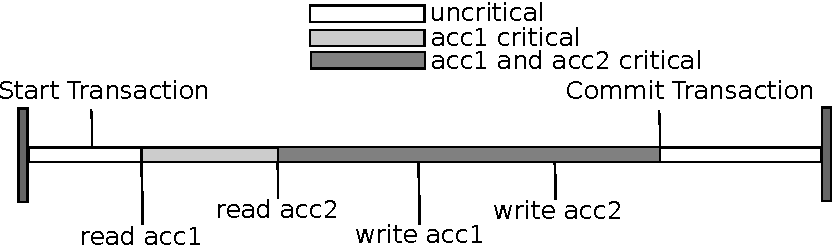
\includegraphics{Figures/CriticalValue}
\decoRule
\caption[CriticalValue]{Time when the update of \code{acc1} or \code{acc2} causes a rollback.}
\label{fig:criticalValue}
\end{figure}

This leads to two questions:
\begin{itemize}
 \item When is it needed to roll back a transaction?
 \item How can we avoid or at least decrease rollbacks?
\end{itemize}
A transaction needs to be rolled back if it is operating on data that is not a snapshot of the current memory. In other words 
if a value has changed after the transaction read this value. When a transaction reads a TVar, this TVar becomes 
\keyword{critical} for the transaction. Critical means a modifications of that TVar causes the transaction to roll back.
Figure \ref{fig:criticalValue} visualizes when the TVars \code{acc1} and \code{acc2} are critical for \code{transaction1}.
When \code{readTVar acc1} is executed the values becomes critical and stays critical until the transaction commits.
If any other transaction commits a modification to \code{acc1} or \code{acc2}, while \code{acc1} and \code{acc2} are
critical for \code{transaction1}, \code{transaction1} is rolled back to preserve the ACI properties. A solution other
than the roll back is presented in \ref{Prob:UnRe}. 

This insight brings an intuitive way to deal with this problem. If we minimize the time the TVars are critical for
a transaction we reduce the chance that this transaction is rolled back. 
If we rearrange the operations of \code{transfer}, we are able reduce the time \code{dst} is critical. Note that we 
can rearrange the operations to a certain degree without changing the semantics of the resulting code due to the ACI 
properties. 
\begin{lstlisting}
transfer src dst am = do 
  srcBal <- readTVar src
  writeTVar src (srcBal - am)
  dstBal <- readTVar dst
  writeTVar dst (dstBal - am)
\end{lstlisting}
With this implementation of transfer the time in that both TVars are critical is reduced. Figure \ref{fig:criticalValue2}
shows the effects of this for \code{transaction1}. The second TVar, namely \code{acc2}, is shorter critical than in the 
initial implementation. The time \code{acc1} is critical has not changed at all. Nevertheless it shows that delaying the
execution of \code{readTVar} can reduce the time values are critical and by this the chance the transaction is rolled back.
\begin{figure}
\centering
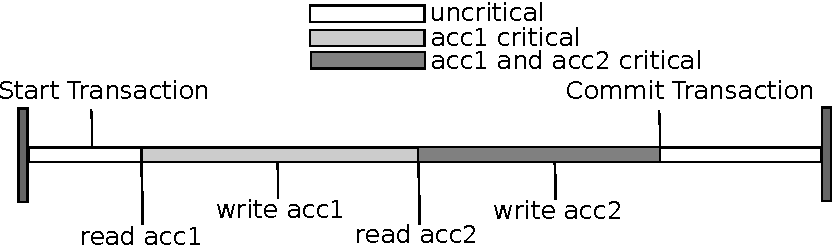
\includegraphics{Figures/CriticalValue2}
\decoRule
\caption[CriticalValue2]{Effect of rearranging code with regards to the time \code{acc1} and \code{acc2} are critical for \code{transaction1}.}
\label{fig:criticalValue2}
\end{figure}
Our aim is to delay the execution of \code{readTVar} as far as possible to reduce to time that
a TVar is critical for the transaction. We have already seen one option to achieve this; rearrange the 
operations of a transaction. This would require a kind of preprocessing in the compiling process, for 
example a source to source code transformation. The aim of this thesis is to provide an pure Haskell
library. I do not intend to implement an extension to the compiler nor do I 
want to provide a source to source code transformer. The only other option is to alter implementation
of \code{readTVar} and \code{writeTVar} without changing the \keyword{external} semantics of STM. 
External semantics are the semantics the user can observe and which effect the user written code.

The critical time would be minimal if the TVars were read directly before or at the start of the commit phase.
This would mean the chances that another transaction commits a change to a TVar that is critical are low or non
existing. So the idea is to let the user define transactions like before, but changing the semantics of 
\code{readTVar} that it is evaluated in the commit phase. The user is able to define transactions like with 
the original implementation, but the delay of the evaluation shortens the time TVar are critical and thus
the chance a transaction is rolled back. 

If we refer to our example: 
\par\noindent
\begin{minipage}[t]{.45\textwidth}
Thread 1:
\begin{lstlisting}[frame=lrtb]
transaction1 = do
  a1 <- readTVar acc1
  a2 <- readTVar acc2
  writeTVar acc1 (a1 - 50)
  writeTVar acc2 (a2 + 50)
\end{lstlisting}
\end{minipage}
\hfill
\begin{minipage}[t]{.45\textwidth}
Thread 2:
\begin{lstlisting}[frame=lrtb]
transaction2 = do 
  a1 <- readTVar acc2
  a2 <- readTVar acc1
  writeTVar acc2 (a1 - 50)
  writeTVar acc1 (a2 + 50)
\end{lstlisting}
\end{minipage}

If we change the semantics of \code{readTVar} by delaying the evaluation, the following happens.
Both transactions will execute the computation phase simultaneously. This means \code{transaction1} adds
\code{(acc1,a1,(a1 - 50))} and \code{(acc2,a2,(a2 + 50))} to its log (this is analog for \code{transaction2}).
At the first glance this seems to be incorrect since the values of \code{a1} and \code{a2} are not yet present.
For Haskell this is quite common. Haskells is a non-strict language, which means passing unevaluated expressions
is normal. 

After the computation phase the commit phase follows. The first step is to lock the read TVars in order to 
perform the validation. Since both transactions used the same TVars, they will commit successively instead of
parallel. 

Assume \code{transaction1} gets the locks first and tries to validate\footnote{You could argue that 
evaluating \code{readTVar} operation is necessary before validating, but this would not change the validity of the 
transaction, since the TVars are locked and can not be modified by other transactions at that point.}. 
Since the readSet contains an action whose result is the current value, the validation is unnecessary; it is always valid.
To validate the log, \code{a} and \code{b} are evaluated. At last the new values are written to the TVars.

After \code{transaction1} finished and released the locks, \code{transaction2} aquires these locks
and validates. The log of \code{transaction2} is also valid and also commits its changes.

Both transactions run parallel as far as possible and did not roll back. Chapter \ref{Chapter2}
presents the limitations of this idea and the challenges that arise when implementing it.

\subsection{Unnecessary Recomputations}
\label{Prob:UnRe} 	
While the first problem dealed with then question \textit{when} transactions need to be rolled back,
the second problem investigates the question \textit{how} transactions are rolled back. Lets take a 
look at our well known example:
\begin{lstlisting}
transfer src dst am = do 
  srcBal <- readTVar src	
  writeTVar src (srcBal - am)	
  dstBal <- readTVar dst	
  writeTVar dst (dstBal + am)	
\end{lstlisting}
This transaction contains two independent statements. The first two lines of the transacton form the first 
statement. This is independent of the last two lines. Independent means their side effects or results do not 
influence each other. While the first line influces the second line, it does not influence the last two lines
and vice versa. 

If the transaction is executed, it computes its log first. Then it locks the TVars and 
validates\footnote{We want study the two problems independently and thus assume the original implementation here.}. 
The validation fails if either of the TVar has changed after it was read by the transaction.
If the validation fails the transcation is rolled back. Which means the log is discarded,
regardless which TVar was the reason for the failed validation. 

Suppose a \code{transaction1} executes \code{transfer acc1 acc2 5} and is deschedules before committing.
Then \code{transaction2} modifies \code{acc1} (and nothing else) and commits. This would cause \code{transaction1}
to roll back and execute both parts of \code{transfer} again. This includes the read and write of \code{t2}, although 
the \code{t2} was not modified. Hence the exact same code with same inputs and the same (relevant) environment 
is executed twice. If we just execute the parts of a transaction that are invalid instead of all, we can save a 
considerable amount of time when a transaction is rolled back. This means for the exmple, it is enough to remove 
the entry for \code{acc1} from the log an execute the first two actions of transfer instead of all actions.

\section{Terminology and Conventions}
To avoid miss understandings, we use this section to define the meaning of specific terms and explain code conventions.

\subsubsection{Conflict}
A \keyword{conflict} in STM is if two transactions access the same TVar in the following way. Transaction t1 reads 
the TVar. After t1 has read the TVar and before it has commited, transaction t2 successfully commits a modification 
to this TVar. This means that t1 works with an outdated value and has to be rolled back. 

\subsubsection{Critical TVar}
A TVar is \keyword{critical} for a transaction t1 if a modification to this TVars causes t1 to roll back. In the current
implementation each time a transaction executes \code{readTVar}, the read TVar becomes critical for this transaction. 

\subsubsection{Deadlock}
The term \keyword{deadlock} is defined in different ways in literature. A deadlock is either a property
of the state of a running system or a property of the source code. In the course of this thesis a deadlock
is a static code property. A program contains a deadlock if there is a schedule that no systems progress is
possible. 

\subsubsection{Code Conventions}
In the code examples givin in this thesis, I often use undeclared variables for the sake of space.
The type of these variables can usually be derived from the context they are used in. Nonetheless, for 
clearity I will give a guideline for naming conventions. In many code examples \code{t1} and \code{t2} 
are used to denote TVars. The type of these TVars depend on the context and is not important for the
examples. The examples that refer to the bank accounts (\ref{STMInterface}) use \code{acc1} and 
\code{acc2}. If \code{t1} or \code{t2} are used to denote transactions, this is always explicitly 
noted in the text. \code{a} and \code{b} denote pure values and are usually introduced in the code.

All code example use the do-notation, which is syntactic sugar for the monadic functions \code{>>=} and 
\code{>>}. In the text that explain the examples, we use \code{>>=} and \code{>>} nevertheless.
In case you are not familiar with do-notation, it is highly recommended to take a look at 
\url{https://wiki.haskell.org/Keywords#do}.

% Chapter 2

\chapter{Concept} % Main chapter title

\label{Chapter2} % For referencing the chapter elsewhere, use \ref{Chapter1} 

%----------------------------------------------------------------------------------------
In this Chapter we will explore an Approach to handle the problem of \keyword{Unnecessary Rollbacks} described in \ref{Prob:UnRo}.
Before we can understand a solution to this problem we need to analyze the technical reason more precisely. 
I was not able to find an satisfying solution for the problem of \keyword{Unnecessary Recomputations}. In 
Chapter \ref{Chapter5} ideas to solve this problem are discussed.

\section{Unnecessary Rollbacks}
Remember the idea given in \ref{Prob:UnRo}. We suggested to delay the readTVar operations to the commit
phase rather than executing them immediately in the computation
phase. While the idea works for the example of a normal \code{transfer}, the idea does not work 
for the following example:
\begin{lstlisting}
limitedTransfer src dst am = do 
  srcBal <- readTVar src
  if srcBal < am
    then return ()
    else do dstBal <- readTVar dst
            writeTVar src (srcBal - am)
            writeTVar dst (dstBal + am)
\end{lstlisting}
If we use this function, the result of \code{readTVar src} is needed in the computation phase and therefore 
the evaluation cannot be delayed to the commit phase. The value is needed to decide the condition of the 
\code{if} expression. To be exact the value is needed to determine the control flow. 

This leads to the question whether there is a way to determine if the result of a \code{readTVar} effects the 
control flow or not. The current implementation does not do this. The main problem is the bind
operator: \code{>>= :: STM a -> (a -> STM b) -> STM b}. This operator allows us to extract the result of an STM action 
from the STM context, for example the result of a \code{readTVar}. This means the STM library loses any possibility to 
observe this value. The value is no longer in the libraries reach. Thus the library is not able to decide if 
the value is used to alter the control flow. Furthermore the library is not able to determine if the control
flow alters when the value is modified. The only way to guarantee the ACI properties is to restart the 
transaction when the TVar is modified. Otherwise the consistency may be violated.

If the library handles a value that is \textbf{not} used for branch conditions as if it were used for branch conditions, 
it may lose performance, but preserves the correctness. We already know an example for this. When we introduced
STM in \ref{STMInterface}, we examined two transactions executing \code{transfer}. In \ref{Prob:UnRo} we detected
that this would roll back at least one of these transactions. 


If the library on the other hand handles a value that \textbf{is}
used for branch conditions as if it were not, the library would not perform unnecessary rollbacks, but may violate 
the ACI properties. Thus GHC handles all values as if they are used for branch conditions to ensure the correctness 
of the implementation. Take for example \code{limitedTransfer acc1 acc2 50} and assume the initial value of \code{acc1} is 60. 
The transaction executes \code{read acc1} (and does not handle this TVar as a critical TVar) and determines the 
branch condition to be false. Then another transaction withdraws \code{20} from \code{acc1}. Afterwards the initial  
transaction resumes and completes its computation phase. Since no TVars are critical the validation succeeds and
the transaction continues. The behaviour depends on the semantics of \code{readTVar}. Either the TVar is read now
(in the commit phase) or the TVar is not evaluated, since it was already evaluated to determine the branch condition.
If the TVar is read again and the update is commited, the new value of \code{acc1} is \code{-10}. Certainly nothing
you expect, when executing a \code{limitedTransfer}. If the TVar is not read again the new value of \code{acc1} is
\code{10}. This is a lost update that generated money. 

\section{Approach}
My approach to avoid unnecessary rollbacks and preserve the correctness is to handle all TVars uncritical, at first. 
While executing the computation 
phase, the TVars whose values are used to alter the control flow become critical. All \code{readTVar} operations are
evaluated as late as possible, meaning a read on an uncritical TVar is executed in the commit phase and a read on 
a critical TVar is executed as soon as its value is used for some kind of branch, by which the TVar becomes critical.

Branch features in Haskell are the following:
\begin{itemize}
 \item \code{if-then-else} expressions
 \item \code{case} expressions
 \item guards in functions or case expressions
 \item pattermatching in functions
\end{itemize}
Whenever a value is passed to one of these constructs, the associated TVars are marked critical
and the affiliated read operations are evaluated. The \textit{associated TVar} are the TVar 
that the value depends on. In other words, the TVars that must be read to determine the value.
A value may depend on multiple TVars. Consider the following example:
\begin{lstlisting}
transaction =
  a <- readTVar t1
  b <- readTVar t2
  if a < 5
    then if b - a < 0 
            then ...
\end{lstlisting}
In this example the value in the condition of the first \code{if} expression depends on \code{a}, but not
on \code{b}. The value in the condition of the second \code{if} on the other hand 
depends on \code{a} and \code{b}. If \code{a} is greater or equal to \code{5}, only \code{t1} is critical
in this transaction, otherwise \code{t1} and \code{t2} are critical in this trasaction. However, the time 
\code{t1} and \code{t2} are critical is different because \code{t1} becomes critical when the first \code{if} 
condition is evaluated and \code{t2} when the second \code{if} condition is evaluated. \code{a} is \textbf{not} 
evaluated again when the second \code{if} condition is evaluated. Every TVar is read at most once per 
transaction regarless the number of branches that depend on the TVar\footnote{It should be clear that the
actual TVars are read again, when the transaction is rolled back.}. Even when the user evokes
multiple \code{readTVar} operations on the same TVar, the actual TVar is accessed just once. 

At the end of the computation phase all reads that are needed to decide the control flow are evaluated. 
%Interestingly this is exactly the case when Haskell demands the evaluation of the values. 
All other reads are not relevant for the control flow and thus not evaluated. 
In the \code{transfer} example no \code{readTVar} is evaluated in the computation phase, because neither of the 
TVars is used to decide the control flow.

Lets refrain from STM and concurrency for a second. This kind of evaluation is well known in Haskell. There 
are two cases where Haskell demands the evaluation of an expression\footnote{There are other cases where Haskell
demand the evaluation, but these are user defined strictness annotation suchs as \code{seq} or \code{!} for strict 
pattern matching or strict constructors. But these are not part of the actual semantics of Haskell.}. 
The first is, if Haskell needs the value to execute a forreign function such as \code{putChar}.
IO actions often contain calls to foreign functions. Although it is not necessary that an IO action calls a 
foreing function and evaluates its subexpressions, every IO action potentially evaluates its subexpressions. 
The second is, if the value is needed to decide a branch condition.

STM is an abstraction that allows us to use sequential programming in a concurrent context. So we can use the 
same evaluation strategy as in the sequential context. Even if the syntax suggests it, we do not explicitly
specify when a TVar is read. We just specify the origin of the value and the evaluation is handled by the 
underlying system. Since the computation phase is processed in the STM monad, there are no IO actions allowed.  
This implies the only time we need to evaluate an expression is when we need to decide a branch condition. 
Everytime we execute other computations on TVar values and write them back or return them, this is not executed 
in the computation phase, because it is not needed. 
By evaluating only the reads that are needed and just before they are needed we minimize the time the TVars are critical. 
Figure \ref{fig:lessCriticalValue} shows the effect on \code{limitedTransfer acc1 acc2 5}\footnote{We 
assume that \code{srcBal} is greater than 5.}. 
\begin{figure}
\centering
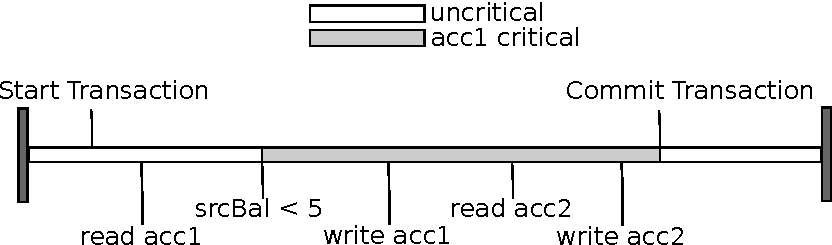
\includegraphics{Figures/lessCriticalValue}
\decoRule
\caption[Less Critical Value]{The critical time of the TVars in \code{limitedTransfer} with the alternative approach.}
\label{fig:lessCriticalValue}
\end{figure}
The TVar \code{acc2} is not critical at any point in the transaction, because it is not needed for the control 
flow. \code{acc1} on the other hand becomes critical at the time its value is used to evaluate the branch
condition \code{(srcBal < am)}.

When the commit phase starts some reads are evaluated and some are unevaluated. Before the remaining
reads are evaluated the transaction acquires all locks for TVars it has modified. Chapter \ref{Chapter3} explains that it 
is enough to lock the TVars that are modfied instead of all TVars that were accessed. Then the transaction is validated.
This validation is similar to the validation in the original implementation; it is a comparision between
the values in the log (the TVars that the transaction needed to read to determine the control flow) and
the current values of these TVars. If all values match, the transaction is valid, otherwise it is invalid.
An invalid transaction is rolled back immediately after the locks are released. If the transaction is
valid, it finally executes the remaining \code{readTVar} operations in order to modify the 
actual TVars and determine the return value of the transaction. Then the modifications the transaction 
performed are committed to actual TVars. By committing the modifications the old values in the TVar are 
overwritten. This is the reason the \code{readTVar} operations can not be delayed any longer. 
Parallel to writing the actual TVars, the locks for these TVars are released. The last step of the transaction 
is to return the result. 

 
% Chapter 3

\chapter{Implementation} % Main chapter title

\label{Chapter3}

We will now look upon the implementation of the aforementioned changes. Unlike to the original
implementation this is not a C library but a pure Haskell library. This brings some advantages 
and one disadvantages. The disadvantage is the performance as discussed in Chapter \ref{Chapter4}.
For the costs of performance we gain a library that is easy to understand and extend. The original 
implementation is interwoven with the GHC runtime environment. Some STM functions are evoked by 
the scheduler to ensure the consistency. This makes the library sensitive to changes. 
To ensure the correctness of such a library is significantly harder than for pure library, since
the compiler does not aid this porcess. In other words, the devlopment of a pure library is safer
and faster. \parencite{STMHigh} presents a high level Haskell implementation of STM. Their aim
was to provide a pure Haskell implementation that is equivalent to original implementation of 
\parencite{STMBase}. Preceding this master thesis I optimized that implementation. I replaced
internally used data structure and performed two changes to the internal semantics. First, 
the initial high level implementation used a global lock to synchronize concurrent transactions.
This coarse grained locking was substituted by a fine grained locking. Instead of a single
global lock, each TVar holds its own lock and transactions acquire the minimum amount of 
locks to commit. This allows transactions that do not conflict to commit simultaneously.
Second, I altered the conflict detection. The initial implementation used a validation process
similar to the GHC implementation. Now each TVar has a queue associated. If a transaction reads 
a TVar, it enters a reference to itself to this queue. If a transaction successfully commits a change to a TVar, it 
notifies all transactions in the associated queue. If a transaction is notified, it is rolled back.
This way of conflict detection has the advantage that conflicts are detected earlier than before.
This implementation is called the \keyword{Project implementation} in the following. Figure 
\ref{fig:implementations} visualizes the development process of the libraries.
We will now head over to a detailed description of the implementation developed in the course of this 
thesis. 

\begin{figure}
\centering
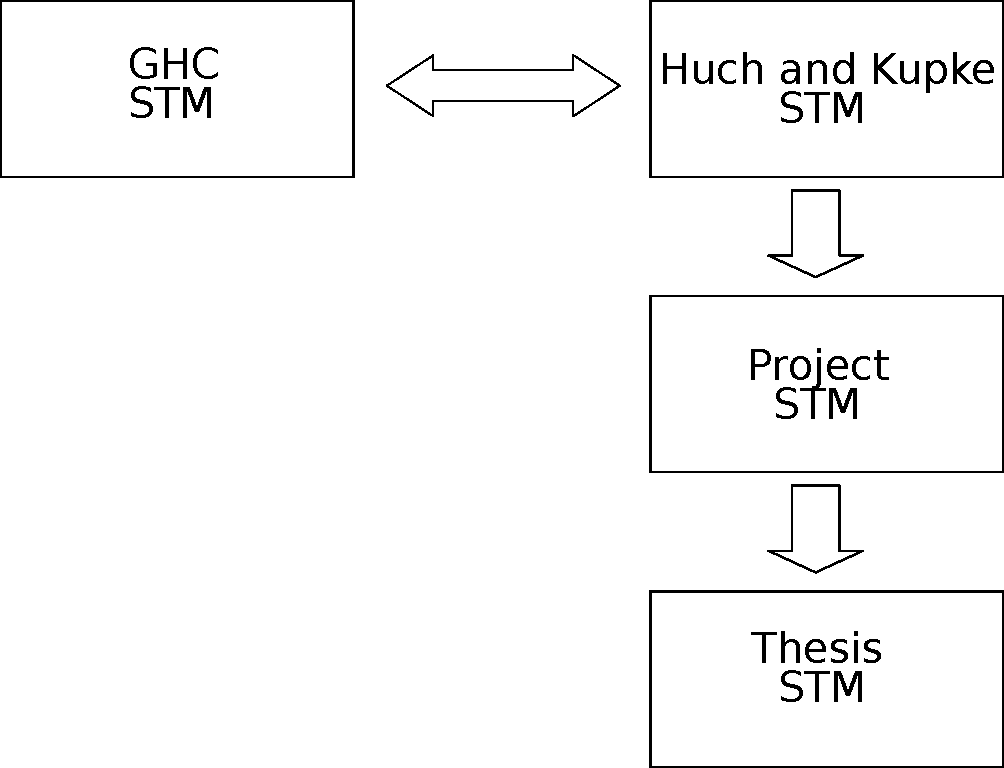
\includegraphics[scale=0.8]{Figures/implementations}
\decoRule
\caption[Implementations]{The STM implementations for Haskell.}
\label{fig:implementations}
\end{figure}

\section{STM Types}
\label{STMTypes}
Before we head over to the implementation of the external interface of STM, we investigate the types
of STM that are used in this implementation starting with the STM type itself:
\begin{lstlisting}
 data STM a = STM (StmState -> IO (STMResult a))
\end{lstlisting}
In its core the STM data type is similar to a state monad. The IO type was initially needed to perform the reads 
in the computation phase. As we will see in the next section, in this implementation it is needed only to create new TVars
in the computation phase. \code{readTVar} and \code{writeTVar} do not need to process IO operations.
Thus an STM action takes a state and returns a result depending on this state. There are three possible 
results:
\begin{lstlisting}
 data StmResult a = Retry StmState
                  | InValid
                  | Success StmState (Maybe a)
\end{lstlisting}
The first constructor is used to indicate that \code{retry} occurred. This must be distinguished from 
\code{InValid}, since \code{orElse} and \code{atomically} react differently on these results. If 
\code{Retry} is returned, \code{atomically} validates and rolls back at an appropriate time; \code{orElse} 
starts the second transaction. This is the reason \code{Retry} is accompanied by the state.
The state holds the necessary information about the TVars that the transaction has read. This allows 
to validate and possibly suspend on particular TVars. \code{InValid} on the otherhand indicates
always that the transaction is not valid and thus must be restarted. 
The last constructor is the desired outcome of an action. If the transaction does not fail, it returns
\code{Success} and a state as well as the result. As before the state is needed for validation.
The result is wrapped with the \code{Maybe} type. The value \code{Nothing} never occurs. 
The reason for this wrapping is explained in Section \ref{sec:IFFun}. 

Before we examine the StmState, we need to take a look at the \code{TVar}
\begin{lstlisting}
 data TVar a = TVar (MVar (IORef a))
                    ID
                    (MVar [MVar ()])
                    (MVar ())
\end{lstlisting}
All TVars have a globally unique identifier called \code{ID}, which is immutable. The \code{MVar (IORef a)} 
holds the actual value of the TVar. The MVar is used to synchronize multiple transaction, if they intend to 
access the same TVar. The \code{IORef} is needed to enable a correct validation, which is explained in detail
in \ref{sec:IFFun}. \code{MVar [MVar ()]} is the queue of the MVar where transactions that wait on a change
enter their their personal \code{MVar ()}. Remember that this is needed to delay the rollback when \code{retry}
is evoked. The last part is an explicit lock for this TVar. There are currently two implementations as 
a result of this thesis. One of these implementations locks a TVar via 
the explicit lock and the other by taking the MVar that holds the value. The details are explained later. 

The computation phase does not allow any observable side effect and its only result is the \code{StmState} and 
a single value.
Hence, the core data structure is the \code{StmState} which holds all informations to commit a transaction:
\begin{lstlisting}
 data StmState = TST {writeSet   :: IntMap (Maybe (),
                                            Maybe (),
                                            MVar (IORef ())),
                      notifies   :: IO (),
                      readSet    :: ReadSet,
                      retryMVar  :: MVar (),
                      uEReads    :: [Maybe ()]}
\end{lstlisting}
The \code{writeSet} is similar to the log in the GHC implementation. Here it is an \code{IntMap} 
\footnote{This refers to the IntMap in the standart libraries of Haskell: \url{https://hackage.haskell.org/package/containers-0.5.8.1/docs/Data-IntMap-Strict.html}}. 
The keys are the IDs of the associated TVars. The elements contain the \code{expectedValue},
the \code{newValue}, and \code{actualMVar}. The \code{actualMVar} is the value holding MVar of the TVar and is needed in the commit
phase when the transaction sucessfully commits to publish its modifications. The \code{expectedValue} 
and \code{newValue} are similar to the log entries presented in \ref{sec:GHCImpl}, but their purpose is slighty 
different. The \code{Maybe} type indicates that the values also can be \code{Nothing}. This holds
only for the second entry. The first entry has the \code{Maybe} type for the same reason 
\code{Success} has it. The second entry on the other hand can become \code{Nothing}. This indicates
that the TVar was read but not written by the transaction. Note that there are two kinds of 
\textit{read}. The first is that a \code{readTVar} operation is porcessed in the computation phase
and the second that the current value of the TVar is read. In the original implementation these 
two occur always at the same time. In the new approach theses kinds of reads occur at different times.
For clearity, from here on I will use IO-reads when I refer to a read from the actual IORef to access
the current value of that TVar. Since Haskell does not provide a simple solution for inhomogeneous
containers, I decided to use the type \code{()} and cast all values via \code{unsafeCoerce} before
entering them to the \code{writeSet}. Whenever a value is taken from the \code{writeSet} it
is casted back to its original type by \code{unsafeCoerce}. The ID of the TVar ensures that 
the type it was casted from does not differ from the type it is casted to.

\code{nofifies} holds an IO action that is process when the transaction successfully commits.
This IO action notifies all transactions that are waiting on a TVar that is modified by the 
committing transaction.

\code{readSet} stores information about the IO-reads that where performed. The type \code{ReadSet}
is defined as follows\footnote{Notice the difference between 
\code{readSet} and \code{ReadSet}. \code{readSet} is the field of the \code{StmState} and 
\code{ReadSet} is the data type.}:
\begin{lstlisting}
 type ReadSet = IORef (InMap (IORef (), 
                              MVar (IORef ()), 
                              MVar [MVar ()]))
\end{lstlisting}
The need for the outermost IORef is explained later. This type is like the \code{writeSet} an 
\code{IntMap}. The keys are the IDs of the TVars. The entries consist of three parts. First,
the value (in form of the IORef) that was present when the IO-read was executed. Second, the 
MVar of the TVars that hold the value. Third, the queue of the associated TVar.
The exact ussage of this is explained in the next section.

\code{retryMVar} is a unique MVar for every transaction. This is the MVar that is entered into
the queues of the TVars when the transactions processes \code{retry}.

\code{uEReads}(unevaluated read) contains all unevaluated IO-read operations. This is essential to be able to 
process the IO-reads that where not evaluated in the computation phase. The \code{Maybe} type
is again used for the same reasons as it is in \code{StmResult}.

This concludes the overview on the data structures used and we can head over to see how these
data structures are used to implement the STM interface.





\section{Interface Functions}
\label{sec:IFFun}
Here we will inspect the implementation of every interface function. 

\subsubsection{newTVar}
\label{sec:newTVar}
This is the only function (besides \code{atomically}) that uses IO actions. A TVar consists of three MVars
and one ID. To ensure the uniqueness of the IDs the STM library defines \code{globalCount :: MVar Int}
and a function \code{getGlobalId :: IO Int} that takes the \code{globalCount}, increments it, writes it back 
and returns the old value. Due to the semantics of the MVar only one thread at a time can get an ID. 
No ID is assigned twice unless \code{globalCount} overflows. Because the chances that this happens 
are narrow, no countermeasures are performed to detect or avoid this problem. 

All MVars are created with \code{newMVar}. This means all MVars are initialized when the TVar is created.
The queue holds and emppty list the lock holds unit and the value hold an IORef with the passed value.
In the end the unchanged state as well as the new TVar is returned.

Lets take a look at the following example:
\begin{lstlisting}
transaction = do 
  tv <- newTVar 5
  a <- readTVar tv
  writeTVar tv (a + 1)
\end{lstlisting}
The first action of this transaction is the creation of a new TVar. This means a new IORef with 
the value \code{5} is created. After that three new \code{MVars} are created. The first contains the 
IORef, the second \code{[]} and the third \code{()}. With a the value gained from 
\code{getGlobalId} a new TVar is created. We assume the ID is \code{1} for now. 
The state on the other hand is not modified. Then the 
second action, \code{readTVar tv}, is processed.


\subsubsection{readTVar}
This function is the core of the new implementation. One part of \code{readTVar} is similar to the original 
Implementation. If the TVar is present in the \code{writeSet}, the \code{expectedValue} is returned (explained together with \code{writeTVar}).
The differences are in the other part of \code{readTVar}. Recall the type of \code{readTVar :: TVar a -> STM a}.
The result is an STM action. This means a function that takes a \code{StmState} and returns an \code{StmResult}. 
Unless the result is \code{InValid}, it contains a \code{StmState}. In other words, \code{readTVar} transforms
the state and returns the value of the TVar. To return the value of the TVar it would be needed to IO-read the
TVar. To avoid this the read is not executed directly. The function \code{buildVal} helps us to achieve this.

\code{buildVal} wraps
the value with \code{unsafePerformIO}. \code{unsafePerformIO} allows us to execute IO actions in pure
Haskell code. These IO actions are executen when the evaluation of the expression that they occur in 
is demanded. In this case the IO action consists of two parts. First, it IO-reads the 
current value of the TVar and returns it after wrapping in into \code{Just}. The wrapping with 
\code{Just} is explained when we examine the implementation of atomically. Second, entering the 
information to the \code{readSet} that are needed to validate. These are the ID of the TVar as 
key, the MVar of the TVar that holds the value, the value that the transaction saw when it IO-reads
the TVar, and the queue of that TVar. The value the transaction has seen in created by the first 
part of the \code{unsafePerformIO} action. The other information are the arguments of \code{buildVal}. After \code{buildVal}
created this wrapping, the expression is (from Haskells view) a normal expression, but the IO-read is
performed when the evaluation of the expression is demanded and not earlier; simultaneously is this 
evaluation logged in the \code{readSet}. Haskell demands the evaluation of values just to decide on
branch condition or to perform IO actions. IO actions are not allowed in the STM monad by the type
system. Thus the evaluation in the computation phase is only demanded when the control flow depends 
on it. 

Back to \code{readTVar}. \code{buildVal} is used to create the result. \code{readTVar} also modifies the 
the \code{StmState}. It adds the newly created value to \code{uEReads}. And it extends the writeSet.
At this point there is no entry for the TVar in the writeSet yet, otherwise this part of \code{readTVar}
would not be executed. A new entry is inserted. This entry contains the constructed value and 
the MVar that holds the value of the TVar. The \code{newValue} field of this entry is \code{Nothing}.
In the end the constructed value and the new state are returned in the \code{Success} constructor.

Reconsider the example givin in the previous section:
\begin{lstlisting}
transaction = do 
  tv <- newTVar 5
  a <- readTVar tv
  writeTVar tv (a + 1)
\end{lstlisting}
We explained already the first action. The first step of the second action is to lookup \code{tv}
in the \code{writeSet}. Since \code{tv} is not present in the \code{writeSet}, \code{buildVal} is
called to create the \code{unsafePerformIO} action. The result (called val in the 
following) is added to the \code{writeSet}. Thus the \code{writeSet} is no longer empty. It contains 
an entry for \code{tv}:
\begin{lstlisting}
 writeSet1 = {(1,(val, Nothing, mvar))}
\end{lstlisting}
\code{mvar} is the MVar of \code{tv} that holds the IORef with the value. The \code{1} is the
ID of \code{tv}. Aditionally is \code{val} 
added to \code{uEReads}. All other parts of the state are unchanged. Due to \code{<-}, \code{val} is 
bound to \code{a} in the end of the second action. 


\subsubsection{writeTVar}
This implementation is straight forward. Two modifications to the state are performed. One is
the modifications on \code{notifies}. A successful commit of the transaction would mean a 
modification to the TVar that \code{writeTVar} was called on. Thus this transaction 
possibly needs to notify waiting transactions. An IO action is created, that notifies
all transactions in the queue of the TVar. This IO action is sequenced by \code{>>} with 
\code{notifies} of the initial \code{StmState}. The resulting action then notifies all
TVars that are written by this transaction. This may lead to an action that notifies the 
same queue twice. This is a minor issue, becuase after the first notification the queue 
is emptied. To avoid this you would need to lookup the value in the writeSet, to see if 
it was already written and if so do not extend the \code{notifies} action. This look up
is most likely more expensive than a notification on an empty queue (this has not been 
investigated). 

The second modification that \code{writeTVar} performs is the modification of the \code{writeSet}.
After wrapping the value for type reasons with \code{Just}, it is entered in the \code{expectedValue} and \code{newValue} 
field of the associated entry in the \code{writeSet}. The last field of the entry is the MVar of
the TVar that holds the value. There is a reason to set both, the first and second field, to the
new value. If the second field is not \code{Nothing}, it indicates that this value is modified 
by the transaction and in the case the transaction sucessfully commits, the value in this field
is written. The first field of the entry is the field that \code{readTVar} returns if it finds
this entry. To avoid this doubled entry, the obvious choice were to use pattern matching to 
check whether the second value is \code{Nothing} and if not return that value. This does not
work in this implementation. The problem is that the pattern matching forces the evaluation.
By forcing the evaluation of an expression you may evaluate IO-reads and thus make TVars critical
that are not critical. This does not happen in the current implementation, because in every entry
of the \code{writeSet} the first field is always not \code{Nothing} and thus can be returned
without pattern matching on this value. 
In the end of \code{writeTVar}, the new state and \code{()} are returned.

For the example it means that the \code{writeSet} and \code{notifies} are modified by the third 
action. The \code{writeSet} looks like this after the third action\footnote{In fact \code{val} 
is of type \code{Maybe Int} and thus cannot be added to \code{1}. The bind operator on \code{STM}
unwraps the value, so we can use it as pure value. This means in the case, that the actual entries are
\code{Just (fromJust val + 1)}. For the sake of comprehensibility, we ignore this for now.}:
\begin{lstlisting}
 writeSet2 = {(1,(val + 1, val + 1, mvar))} 
\end{lstlisting}
In both, the first and the second field, \code{(val + 1)} is entered. \code{notifies} is 
initially \code{return ()}. After the \code{writeTVar} action it is:
\begin{lstlisting}
 notifies1 = do
    queue <- takeMVar waitQ
    mapM_ (flip tryPutMVar ()) queue
    putMVar []
    return ()
\end{lstlisting}
\code{waitQ} is the queue of \code{tv}. The notification is performed by trying to put \code{()}
to the MVars in the queue. It is important to use \code{tryPutMVar} instead of \code{putMVar}.
Otherwise the implementation contains a deadlock (imagine two transactions try to notify the same 
transaction at the same time). In the end the queue is emptied to avoid another transaction to 
notify the same transactions again. The final \code{return ()} is the initial value of 
\code{notifies}. The result of the three action in the example is:
\begin{lstlisting}
 Success state ()
\end{lstlisting}
\code{state} is a \code{StmState} that contains \code{notifies1}, \code{writeSet2} and the 
modified \code{uEReads}. The \code{readSet} and \code{retryMVar} are similar to the one 
in the initial state. This state is used in atomically to commit the changes.


\subsubsection{atomically}
This is the heart of every STM implementation in Haskell; it allows the user to execute STM 
actions in a transactional manner. Before \code{atomically} starts the computation phase, it
creates an initial state. This state basically holds no information and commit with this state
would result in no change at all. After the initial state is created, the computation phase starts. 
In this phase atomically does not do anything but pasing the initial state to the STM action.

After the \code{StmResult} is calculated, atomically starts the commit phase by interpreting
the result. There are three possible outcomes.
First, the result is \code{InValid}. If this occurs the computation phase is just restarted 
with the initial state\footnote{Actually the \code{readSet} needs to be discarded explicitly,
because it is an IORef and thus would not be empty by taking the initial state.}. 

Second, the result is \code{Retry newState}. This casues the transaction to lock the TVars in its 
\code{readSet} which can be accessed via \code{newState}. After the locks has been acquired, 
the \code{readSet} is validated. If it is not valid, the locks for the TVars are released and
the transaction is rolled back like it was done for \code{InValid}. If the transaction is 
valid, the transaction enters its \code{retryMVar} to the queue of the TVars it has read.
These queue are stored in the \code{readSet}. Then the transaction realeases the locks and 
executes a \code{takeMVar} on its \code{retryMVar}. This lets the transaction suspend until
another transaction notifies it. After the transaction was notified, it removes its 
\code{retryMVar} from the queue (if that has not already happend) and restarts.

Third, the result is \code{Success newState result}. This is the most interessting case, 
because it is the commit phase and thus leads not necessarily to a rollback, in contrast to 
the other two results. 
There are currently two different implementation as a result of this thesis which 
only differ in this part. The performance tests presented in Chapter \ref{Chapter4} do
not provide a clear result on which implementation is better in general. I will present
both implementation. When is it not clear which of the implementation we are talking about,
we will refer to the first implementation as STMLA (STM lock all) and the second STMWSL 
(STM write set lock). 

STMLA starts the commit phase by locking all TVars is has accessed. This implementation 
uses the explicit locks of the TVars. This information are 
stored in the \code{writeSet}, since \code{writeTVar} as well as \code{readTVar} create
entries for that are not part of the \code{writeSet}, but processed by either of these 
functions. When all locks are acquired, the transaction validates its \code{readSet}.
If this is not valid, the transaction is rolled back.
If it is valid, the transaction evaluates all expressions in \code{uEReads}. This is done
by the \code{seq} function, which forces the evaluation of its first argument and returns 
its second argument. As always in Haskell the expression is evaluated to WHNF\footnote{In 
case you do not know what \keyword{weak head normal form} is please refer to 
\url{https://wiki.haskell.org/Weak_head_normal_form}}. This is where the \code{Maybe} type 
comes in handy. \code{buildVal} created a \code{Maybe} value that was wrapped with an
\code{unsafePerformIO} action. If we force the evaluation of this expression, the 
IO-read is performed, but the underlying expression is not evaluated, because it is wrapped 
in the \code{Just} constructor. Without this constructor, we would evaluate the expression that 
is stored in the TVar. Imagine this expression is a complex computation. This means, we 
suffer a performance overhead because the computation is not yet needed (even worse if the
computation is not needed at all). 
Even worse we execute this in the commit phase, while we hold the locks for many TVars.
To maximize parallelism, we aim to minimize the time in the commit phase. Besides these
performance problems, there is a serious semantic problem. Everytime we force the 
evaluation of an expression that is not needed, we change the semantics of the program.
This may lead to exceptions or loops that would not occur normaly.
After the \code{uEReads} are evaluated, the actual writes are prepared. The writes are 
divided in two parts. First take the value from the MVar and second write the new value.
Preparing means all the value holding MVars of all TVars that are going to be written
are emptied. Then the \code{notifies} are processed. At last the new values are written
to the value holding MVars. This is needed to prevent a very nasty bug \footnote{For 
interessted readers is this bug explained in the appendix.}. 
The last step of the commit phase before returning the result is to realease the locks
that were taken at the start of the commit phase.

The second implementation (STMWSL) starts the commit phase by validating. As before, the 
transaction is rolled back if it is invalid. If it is valid, the remaining reads in 
\code{uERead} are evaluated. After all reads have been processed, the actual writes are
prepared. This means the TVars that are modified by the transaction are accessed and
their value holding MVar is emptied. At this point no other transaction is able to 
either read or write these TVars. In the first implementation the explicit locks 
were taken, which does not prevent other transactions from reading these TVars.
When the writes are prepared, the transaction is validated again. In contrast to 
the first validation, this validation is mandatory. It is possible that the current
values of the TVars have changed after the reads were processed and before the 
writes were prepared (and by this the TVars locked). The first validation is
added to avoids the problem that the transaction acquires the locks, although it 
is invalid. The costs for locking are much higher than the costs for validation.
If the transaction is invalid after the reads are processed and the transcation
acquired the locks, it is rolled back. If it is valid the it is similar to
the first implementation (STMLA). At first the \code{notifies} are processed
and then the writes are processed. At last the result is returned. Note that
it is not necessary to unlock the TVars explicitly, because only the value 
holding MVars of the TVars serve as a lock in STMWSL. By filling these MVars
the associated TVar is unlocked. 

Both implementation have their own benefits. STMLA does never roll back,
when the transaction does not branch at all. If two transactions read the
same TVar they cannot commit at the same time in STMLA. In STMWSL it is
possible that two transaction, that read the same TVar, commit simultaneously
(if non of them also writes this TVar). It is also possible
that a rollback occurs, even if the transaction does not branch. The 
problem is that the remaining reads are evaluated in an unlocked context.
This means that other transactions can modify these values after they were 
read and thus invalidate the reading transaction. It would be better, if the
transaction process the \code{uEReads} after it has locked the TVars. This is 
currently not possible. As we will discuss in detail in the next section, when 
we only lock the modified TVars, it is essential that no other transaction 
reads them while we hold the locks. Otherwise the ACI properties cannot be 
guaranteed. If we take the value holding MVars it prevents other transactions
from reading the associated TVars. Unfortunately, this also prevents us from 
reading the TVars. That is why we need to process \code{uEReads} before we 
acquire the locks for the TVars. The clever reader may have noticed that 
we get the values of the TVars when we prepare the writes, because we execute
\code{takeMVar} on the value holding MVars. To use these information would 
require the \code{unsafePerformIO} actions produced by \code{buildVal} to 
behave diffrently when it is executed in the computation phase and in the 
commit phase. Nevertheless, this topic remains for future work and is discussed 
in Chapter \ref{Chapter5}.

A solution that combines STMLA and STMWSL would be better\footnote{This could 
not be proved, because no such implementation is present currently.}.
A combined solution locks the TVars that the transaction has modified in a 
manner that no \textbf{other} transaction can read them. The transaction itself
is still able to read the locked TVars. Then the transaction is validated. 
If it is valid, the remaining reads are processed and the transaction publishes
its modifications. At last the transaction returns the result, after unlocking
the TVars.

If we execute \code{transaction} introduced in Section \ref{sec:newTVar} with 
\code{atomically} (of STMLA), the computation phase produces the previously mentioned state.
This \code{writeSet} in this state contains a single entry. The entry for the
newly created TVar. The commit phase starts by validating the \code{readSet}. 
Since the \code{readSet} is empty, the validation succeeds and the transaction
acquires the lock for \code{tv}. After the lock is acquired, the transaction 
evaluates \code{uEReads}. \code{uEReads} contains one value, namely \code{val},
the {unsafePerformIO} action that reads \code{tv}. The evaluation of this value 
has (thanks to sharing) an effeect on the \code{writeSet} as well:
\begin{lstlisting}
 writeSet = {(1,(Just (5 + 1), Just (5 + 1), mvar))} 
\end{lstlisting}
The next step in to prepare the writes. This means \code{mvar} is emptied via 
\code{takeMVar}. Before it is filled again, \code{notifies} is executed. \code{notifies}
does nothing because the \code{waitQ} of \code{tv} is empty. Finally the expression (\code{5 + 1})
written to \code{mvar}. Note that the expression itself is not evaluated. The last step
before returning \code{()} is to release the lock for \code{tv}.

\subsubsection{>>=}
The monadic bind operator, \code{>>=}, is an important part of the interface, because it allow us 
to use the do-natation. The aim of this thesis is to provide an alternative STM 
implementation for Haskell without altering the semantics or interface. One of 
the most comfortable things about is the way we use it. Thus it is important to 
retain this feature. \code{>>= :: STM a -> (a -> STM b) -> STM b} allows us to 
extract the result of an \code{STM} action from the STM context and use it to create 
a new STM action. Additionally it is used to translate \code{<-} of the do-notation.
The implementation is straight forward, but for the sake of completeness presented
nonetheless. The result is a STM action, meaning that it is a function that takes 
a \code{StmState} and its result is a \code{StmResult}. Thus the function basically
has three arguments. The \code{STM} action, the function of type \code{a -> STM b},
and the \code{StmState}. These arguments are called \keyword{passed action/function/state}
in the following. 

The resulting function first applies the passed state to the passed action. 
If the result is \code{InValid}, it just returns \code{InValid}. If it is
\code{Retry newState} it returns \code{Retry newState}. 

Note that it is important to 
pass the \code{newState} created by the action, because it contains information that
are needed to wait before rolling back. 

If the result of the action is 
\code{Success newState res}, the function first needs to unwrap \code{res}; it is wrapped with 
the \code{Just} constructor. This is done by the partial function \code{fromJust}. The
implementation ensure that \code{Nothing} can never occur and thus the call to 
\code{fromJust} is safe. After the value is extracted, it is applied to the passed 
function. This application results in an \code{STM} action. To gain the \code{StmResult} as 
the result of the function the \code{newState} is applied to the action.
Thanks to the laziness of Haskell the call to \code{fromJust} is not evaluated 
immediately. This is the key of this implementation, since we avoid the evaluation of 
the IO-read by this. If \code{fromJust} would be evaluated when the bind operator is evaluated,
a action like \code{a <- readTVar t1} would not differ from the original implementation,
because the \code{unsafePerformIO} action would be executed immediately. 
Since we use a \code{case} expression to branch on the different \code{StmResult}s, we 
could also extract the value from the \code{Maybe} type  via pattern matching instead 
of \code{fromJust}. This would also lead to the evaluation of the value and 
make the wrapping performed by \code{buildVal} futile.

\subsubsection{retry and orElse}
The implementation of \code{retry} and \code{orElse} are very simple. 
\code{retry} is a STM action. The passed state is wrapped with the \code{Retry} constructor.
That is all \code{retry} does. 

\code{orElse} executes the first acion with the passed state and if the result is not 
\code{Retry newState} it just returns this result. If it is \code{Retry newState},
the second action is executed with the passed state (not the \code{newState}) to discard the 
writes executed by the first action. Since the \code{readSet} is an \code{IORef}, 
we do not lose the information on the TVars that was read. 



\section{Notes on the Implementation}
Some details of the implementation remained unexplained until here. These details are highlighted
in this section.

\subsubsection{Deadlock Avoidance}
One Motivation for STM is the deadlock freedom. We have seen in Section \ref{STMInterface} that acquiring 
multiple locks always includes the danger of deadlocks if multiple threads work concurrently. 
There are two concepts to avoid deadlocks for such settings. The setting is that multiple threads
try to acquire and arbitrary number of shared locks. The first avoidance strategy is, if thread tries to 
acquire a lock that is not available, the thread releases all locks and tries to acquire all locks again.
This is continued until the thread can acquire all desired locks. The other avoidance strategy is to 
acquire the locks in a global order. STMLA as well as STMWSL use the latter. The TVars that need to be 
locked are stored within \code{IntMap}s. If a transaction trys to lock these TVars, the transaction converts 
the \code{IntMap} to a list and process it. Since the conversion from an \code{IntMap} constructs an ordered 
list, the transactions always locks in a global order. The TVars are ordered by their IDs.


\subsection{STMWSL}
The double validation of STMWSL seems to be an unnecessary overhead. However, the original implementation 
also uses this scheme, which was proposed by Fraser \parencite[Page 42]{lockfreedom}. The high costs for locking the TVars
are the reason. This locking itself is not particular expensive, but it hinders parallelism.
Everytime a TVar is locked no other transaction is able to read, lock, or validate this TVar. Additionally if 
a transaction tries to access a locked TVar, it is suspended and a context switch follows. Context switches in Haskell 
are not as expensive as context switches of OS threads, but it schould not be neglected, especially when dealing
with a large number of threads. Validation is a operation, which needs two memory access per entry in the log.
One memory access is the access to the log entry to look up the expected value and the other memory access is
the access to the actual TVar\footnote{The log entry needs to be accessed two times. First to get the expected
value and second to get the next entry, because the log is a dynamic structure and thus needs a pointer
to the next entry comparable to a list. Nevertheless the entry itself is (most likely) in one block in the memory.
This is why I consider one memory access to be enough for the entry.}. This is reasonable considering that the 
log only consists of TVars that are needed to determine the control flow. So validation is significant faster
than locking. 



%
\chapter{Evaluation} 

\label{Chapter4}
In this chapter we elaborate the impact of the implemented changes on the performance.
Evaluating STM is worth a thesis itself. The biggest advantage of STM in usability is
its biggest disadvantage in (performance) testing STM. STM is a universial tool. Most
synchronization problems can be tackled with STM. This on the other hand means there
is no clear way to test STM, especially when measuring the performance. Thanks to
the moderate interface, testing the correct behaviour of STM is practicable. Testing 
is no guarantee that the implementation is correct in all regards, but it narrows the 
space for bugs. Due to the small interface of STM the complexity is limited. 
I wrote a number of small tests to test the implementations for specific bugs. Even if 
tests are no guarantee that the implementations are free of bugs, they test a braod portion
of the functionality and reduce the space for bugs. However, we will not investigate these 
correctness tests.


Unfortunately, testing the performance is extremely difficult. There are unlimited 
possibilities to use STM. Thus it is not possible to test the performance in general.
We can only test the performance for specific cases. This makes it hard to say which 
implementation has the best performance in general. To be able to classify the differnt 
tests and to compare the differnt test to each other, we use the following properties: 
\begin{itemize}
 \item costs of a transaction
 \item level of currency
 \item number of branch dependend TVars 
\end{itemize}
The \keyword{costs} of a transaction denotes the time the transaction needs to execute when no 
other transaction is present.  
It is important to distinguish this from the time the transaction needs to execute. The
time heavily depends on other transactions. When a transaction is executed in a system
with many other transaction that work on the same TVars, the chance that it is rolled 
back is higher than if the transaction is the only transaction in the system. In contrast, the costs
of the transaction does not depend on the level of concurrency.

The \keyword{level of concurrency} denote the density of the TVar usage. A high level of 
concurrency is givin if there are many transactions and if these transactions write and read the same
TVars. Read-only TVars are not considered, because reading them cannot result in a rollback.
If every transaction works on different TVars, there is no concurrency at all. If there 
is only one transaction, there is also no concurrency. Thus only if both requirements are satisfied,
we speak of a high level of concurrency. 

The last property is relevant only for the alternative implementation. It denotes the amount of TVars that 
are critical in the new implementation. In the GHC implementation as well as in the implementation
this thesis is based on, all TVars that are read are critical. In this implementation only TVars the 
transaction branches on are critical. 

These properties are not statically measurable, because they often depend on the state of the TVars. 
The cost may vary depending on the branches that are taken. The level of concurrency may also 
depend on branch conditions, because it determines which TVars are accessed. Furthermore does 
the scheduler affect the level of concurrency. The GHC runtime system uses the \keyword{round robin}
scheduling scheme. If all transactions are sufficient cheap, they finish before their time expired.
This means irrespective of the number of threads, there is no concurrency at all (if a single OS thread
is used). The number of critical TVar may also depend on the state due to nested branches.
Nevertheless, we use these vocabulary in the following sections.

\section{Test Setup}
Before we head over to the results, we will look upon the tests that where used to measure the performance.
I used basically two tests to compare the different implementations. The frist test is called \keyword{StmTest}.
It is used to test the performance and the correctness at the same time. StmTest has four parameters to control
the costs of a transaction and the level of concurrency:
\begin{itemize}
 \item threads
 \item iterations
 \item tvars
 \item changes
\end{itemize}
\code{threads} determines the number of threads that are working parallel. \code{iterations} is the number of transactions
each thread executes. \code{tvars} is the number of TVars that are created and used. \code{changes} is the number of 
operations per transaction. I will use these parameters in the following as variables for numbers.
The starts by creating \code{tvars} TVars. Then \code{threads} threads are created. Each thread chooses randomly \code{changes} TVars from all 
created TVars (the same TVar may be chosen multiple times). Then the thread reads each of theses TVars, increments their
value and writes the new value back to the TVar. This is repeated \code{iter} times. When every forked thread has finished the
main threads reads all TVars an sums their values. If the STM system is correct, the sum is (\code{threads * iterations * changes}).

By altering the parameters the level of concurrency and the costs per transaction can be controlled. More \code{threads} and less 
\code{tvars} result in a higher level of concurrency. More \code{changes} mean not only higher costs of a transaction, but also
a higher level of concurrency. Unfortunately, in this test we are not able to increase the costs per transaction without increasing
the level of concurrency. The overall runtime of the test can be managed with \code{iterations}. 
This test clarifies the previously mentioned problem of testing STM. These parameters can arbitrarily chosen and all of the results
are correct uses of STM. The number of combination on the otherhand is nearly unlimited. Thus it is not possible to compare the 
implementations with all possible configurations. To determine which STM implementation is the best overall is anything but trivial.
Nevertheless we use this test to compare the implementation on specific configurations to see their individuel strengths and weaknesses.
Note that the transactions in this test always write all the TVars they have read. This is not necessarily the case when STM in practise. 
That is why I created a second Test to meassure the performance.

\keyword{PerformanceTest} is a test to meassure the performance and not the correctness. In contrast to StmTest is has not four but
five parameters:
\begin{itemize}
 \item threads
 \item iterations
 \item tvars
 \item rWRatio
 \item writes
\end{itemize}
The first three parameters are the same as in StmTest. \code{rWRatio} determines the ratio between reads and writes. For example, if
the \code{rWRation} is \code{5} it means each transaction performs five reads for each write. \code{writes} on the other hands specifies
the number of writes that are executed in each transaction. This test allows us to increase the costs of the transactions by 
increasing the level of concurrency only slightly. If multiple transactions read the same TVar there is no conflict. If multiple
transaction on the other hand read and write the same TVar, there is a conflict. 

PerformanceTest ist similar to StmTest. It first creates \code{tvars} TVars. Then it forks \code{threads} threads. Each of these 
threads creates ramdomly \code{writes} lists with \code{rWRatio} TVars each. For each inner list the transaction reads all TVars,
sums their values and writes them back to the first entry of that list. The list of lists is processed in a single transaction. 
This procedure is repeated \code{iterations} times. Since the TVars are choosen randomly, we cannot determine if the final state
of the TVars are correct after all threads are finished. Another difference between the two tests is that StmTest uses a list to 
store and lookup the TVars, while PerformanceTest uses an \code{IntMap}.

To meassure the performance of the implementations the unix \code{time} command was used\footnote{\url{https://en.wikipedia.org/wiki/Time_(Unix)}}.
The test (either StmTest or PerformanceTest) were compiled with GHC 8.0.1\footnote{\url{https://www.haskell.org/ghc/download_ghc_8_0_1}} and the 
compiler flags \code{\-O2} for optimizations and \code{-threaded} to allow threaded runtime. The test was exectued with the runtime option \code{-N} 
to allow multiple (in my case four) OS threads. The tests were executed on a system with an Intel(R) Core(TM) i7-6500U CPU @ 2.50GHz,
8GB @ 1600 Mhz DDR3 and a Fedora 25 OS. 


\section{Results}
We will now inspect the results of the performance tests. I performed two series of tests to compare the different implementations.
In the first series the tests are configured by hand and the level of concurrency as well as the costs per transaction are modified.
The total workload was the same in all tests in this series. In the second test series the number of threads are increased in every
test. The workload per thread is unchanged and thus the total workload increases with the number of threads. 

\subsection{First Test Series}

\begin{figure}
\centering
 \begin{tabular}[center]{|c|c|c|c|c|}
  \hline
	                     & GHC    & Project & STMLA  & STMWSL \\ \hline
  StmTest(20,1000,200,50)    & 3.2978 &  3.5645 & 3.5340 & 3.6655 \\ \hline
  StmTest(20,2000,200,25)    & 3.3845 &  3.5700 & 3.6335 & 3.6665 \\ \hline
  StmTest(20,0500,200,100)   & 3.1780 &  3.8540 & 3.5905 & 3.7910 \\ \hline
  PerTest(20,500,200,10,10)  & 3.0420 &  3.2830 & 2.9225 & 3.4920 \\ \hline
  PerTest(20,500,200,20,5)   & 3.0670 &  3.3110 & 2.9425 & 3.4445 \\ \hline
  PerTest(20,500,200,5,20)   & 3.1520 &  3.4335 & 2.9455 & 3.3500 \\ \hline
 \end{tabular}
\caption[Runtime: Performance Tests]{Average runtime in seconds for tests with a total workload of 1.000.000 \code{readTVar} operations.}
\label{fig:results1}
\end{figure}

The results of the first test series are shown in Figure \ref{fig:results1}. 
The first column contains the test and its configuration.
StmTest(threads,iterations,tvars,changes) means the \code{StmTest} was applied with the previously explained configuration parameters.
PerTest(threads,iterations,tvars,rWRatio,writes) is the same for \code{PerformanceTest}. The first row introduces the different 
implementations. GHC is the current library in GHC 8. Project is the highlevel library that this thesis is based on.
STMLA and STMWSL are described in the previous chapter. For unknown reasons STMWSL performs poorly in this tests.

In the first three tests we examined how changes in the costs of a transaction effects the runtime of the four systems. 
The number of threads and TVars are fixed. By altering the \code{changes} parameter, we increase the workload per 
transaction. To preserve the total workload, we decrease the number of iterations each time we incease the number
of changes per transaction. In the first test we see that all libraries perform equally good, except for the GHC 
library, which performs slightly better. In the second test the workload per transaction is halved compared to the
first test. The runtime of the GHC library and STMLA raises. The GHC library is the fastest and the thesis libraries 
are the slowest. The third test examines the other direction. The workload per transaction is doubled compared to the 
first test. This leads to an significant increase in runtime for the Project library and STMWSL. The GHC library becomes 
faster with this configuration and STMLA remain on a equal level. This is the result we expected, since the rollback of 
a transaction is more expensive than in the first test. Fortunately does not perform any rollback in this test. The Project
library on the otherhand performs rollbacks, which explains it increase in runtime. GHCs library also performs rollbacks
and thus its increase in runtime is only natural. We additionally increase the level of concurrency by increasing the 
TVars that each transaction accesses, which leads to more rollbacks in the GHC and Project libraries.

The last thress tests use \code{PerformanceTest}. The number of reads per transaction were equal in all tests, but the 
rWRatio was different. In other words the costs of a transaction is modified slightly, but the level of concurrency
is modified greatly. By altering the number of read, we increase the costs of a transaction, but more importantly we 
increase the level of concurrency, because when a transaction writes a TVar another transaction can become invalid.
Thus, the more TVars each transaction writes the higher in the level of concurrency. The first test executes ten writes
per transaction and ten reads for each write. The results are positive for the STMLA, since it is the fastest implementation.
STMWSL is the slowest implementation. The GHC implementation is slighty slower than STMLA but noticeable faster than the 
Project implementation. If we compare this to the second test, where the number of reads remains the same, but the number of
writes is halved, no considerable changes are observed. All implementations remain on a similar level compared to the first
test. If we on the other hand increase the number of writes while retaining the number of reads, the runtime of the
GHC and Project implementations are increasing. The runtime of STMLA remains the same and is like in the two previous 
tests the fastest. Interestingly is the runtime of STMWSL lower than before, but still not comparable to the runtime of
STMLA.

While the results of the first three tests seems not very promising for the need of the alternative implementation, the results
of the last three tests reveal an application where STMLA outperforms even the GHC implementation, which is an omptimized low 
level \code{C} implementation. More importantly, these tests met the expectations regarding the costs per transaction. First,
the performance does not decrease if we increase the costs per transaction. Since we do not execute any rollbacks in these 
tests, the costs per transaction do not matter for STMLA (and STMWSL). The GHC and Project library on the other hand 
lose performance in these cases. Second, the performance does not change if we increase the level of concurrency. By increasing
the level of concurrence the amount of rollback that are executed by the GHC and Project library are increased. STMLA and STMWSL
on the other hand do not suffer from the increased level of concurrency. 
An explanation and a possible solution for the poor performance of STMWSL is givin in Chapter \ref{Chapter5}.


\subsection{Second Test Series}
We use the second test series to study the scalability of the implementations. We use \code{StmTest} as well as
\code{PerformanceTest} to compare the four implementations. Similar to the previous test series, the same test
is executed multiple times and the average execution time is meassures. The tests are randomized by the test themself 
and the scheduler. To get a representative result for the runtime, it is inevitable to execute the test multiple 
times. To test the scalability we increased the number of threads over the course of the series. The other 
configuration parameters remained untouched over the course of the whole test series. 
\begin{figure}
 \centering
 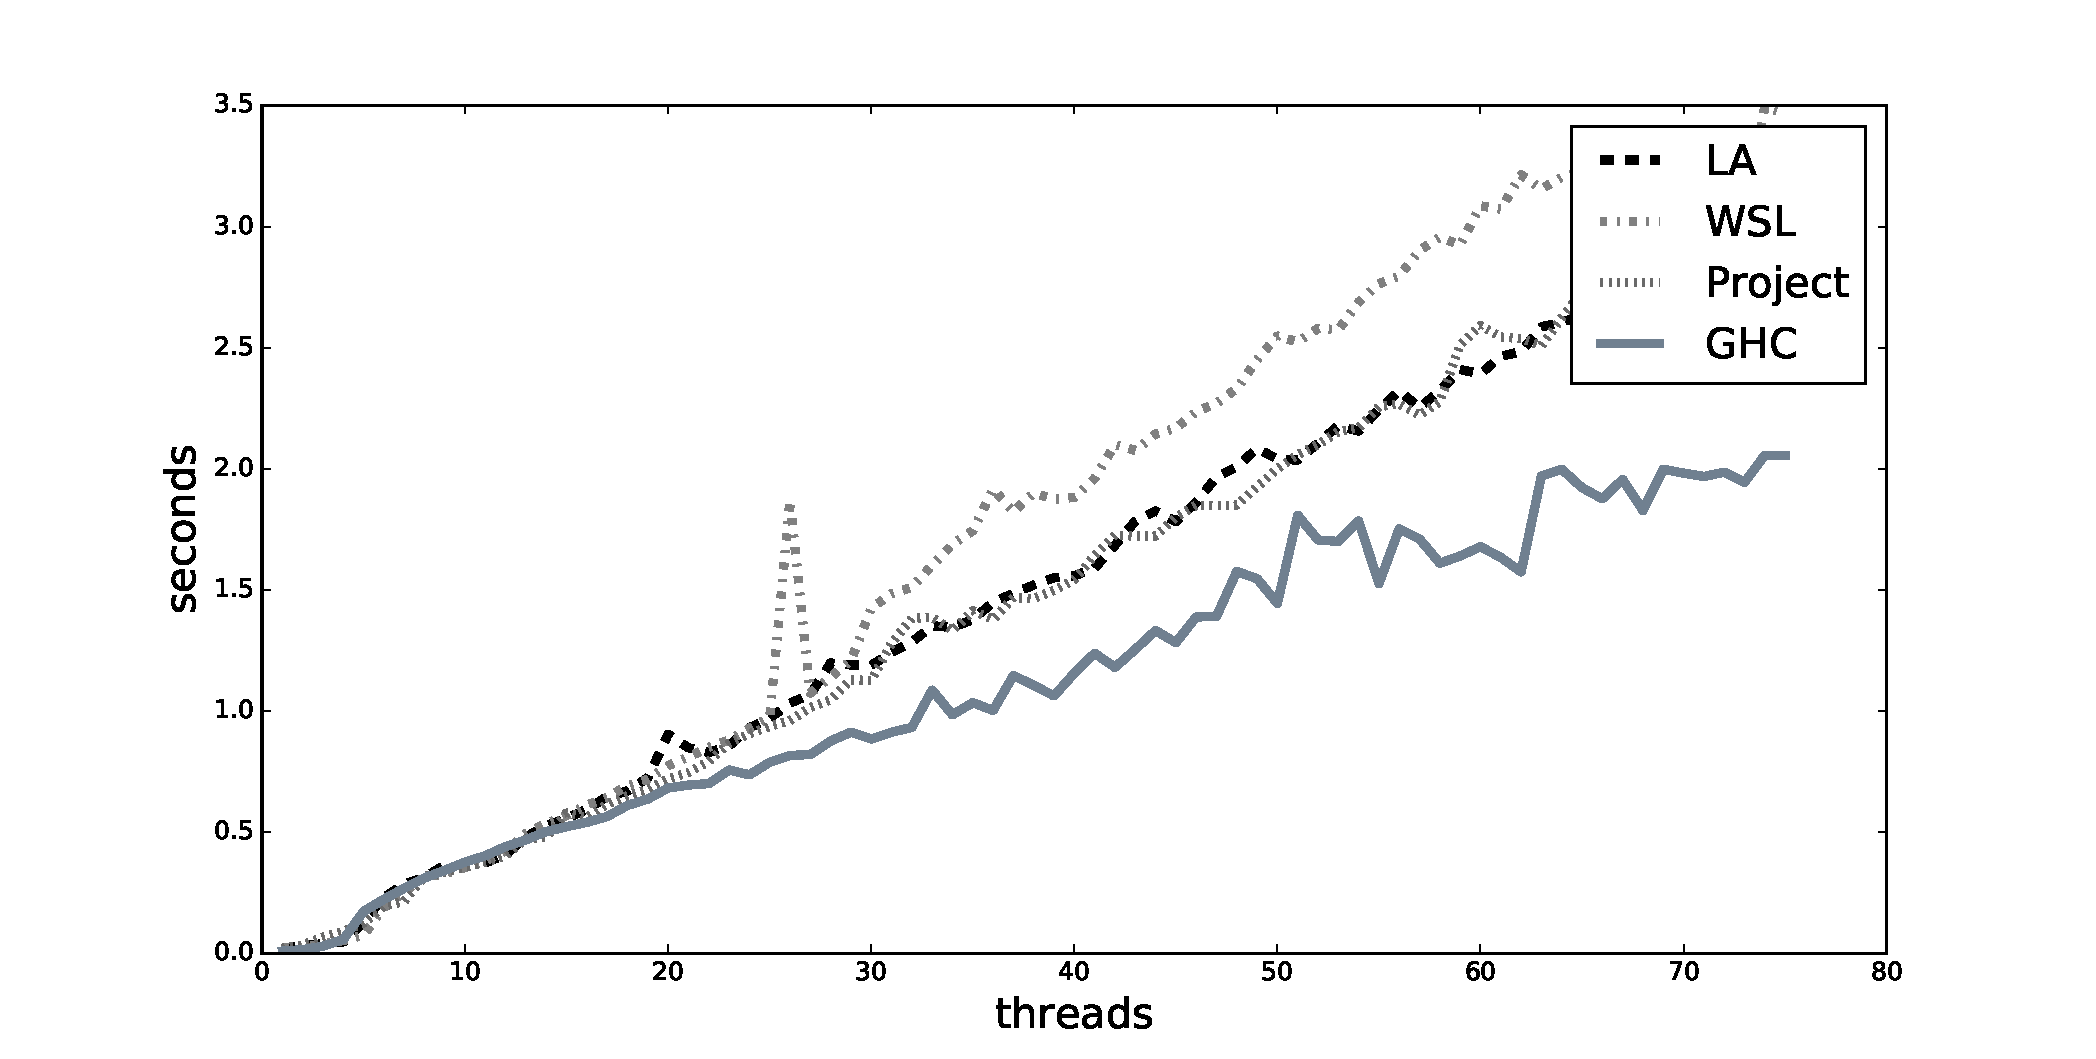
\includegraphics[scale=0.4]{Figures/Scaling1}
\caption[Runtime: Scaling Test I]{Results of the scaling tests with \code{StmTest}}
\label{fig:scaling1}
\end{figure}

Figure \ref{fig:scaling1} show the result of the scaling test performed with \code{StmTest}. We used the following 
configuration: 500 iterations per thread, 100 TVars stored in a list and 20 modifications per transactions with 
a varying number of threads. The x-axis describes the number of threads, while the y-axis contains the total runtime.
Note that an increase in thread results in an increased total work load. The means the increase in runtime in all implementation
is not only due to the fact that the level of concurrency is increased but also due to the increase of the total workload.
All implementations scale equally. The GHC implementation is slightly better and STMWSL is slightly worse than the other 
implementations. Overall, increases the runtime linear with number of threads. The GHC implementation stands out because of
its unstable execution time in this test series. Nevertheless, it still performs better than the other implementations.

\begin{figure}
 \centering
 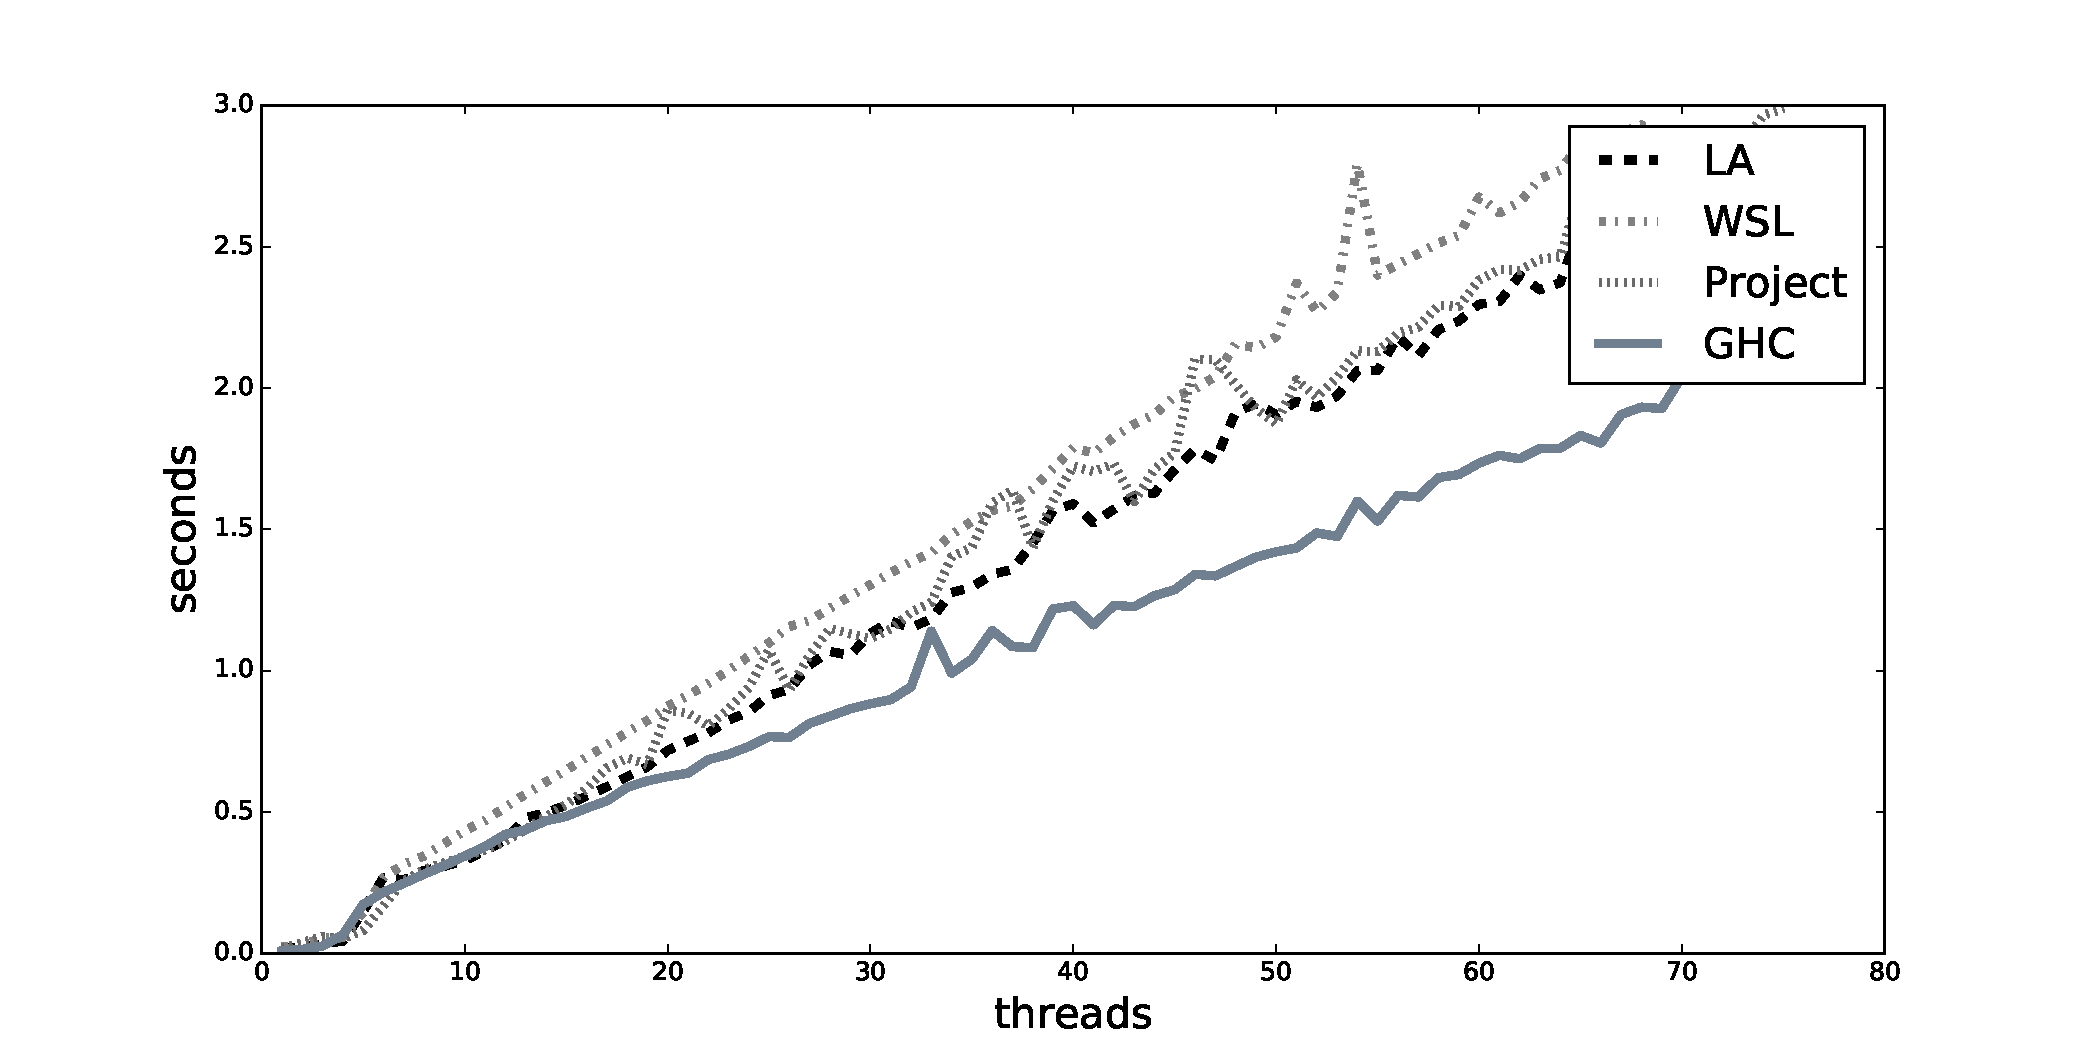
\includegraphics[scale=0.4]{Figures/Scaling2}
\caption[Runtime: Scaling Test II]{Results of the scaling tests with \code{PerformanceTest}}
\label{fig:scaling2}
\end{figure}

The results of the scaling tests performed with \code{PerformanceTest} are presented in Figure \ref{fig:scaling2}. The configuration 
is as follows: 500 transactions per thread, 200 TVar stored in an \code{IntMap}, five times more reads than write and
five writes per transaction (25 read operations per transaction). The results are similar to the previouse results. All implementation scale on equally while
GHC is a slightly faster and STMWSL slightly slower. The differences in the execution time of GHC are less noticable than 
in the first test. The execution time of the project implementation on the other hand varies much more in this test than
in the first test. Nonetheless, the general tendencies are not different. 

This test series show that all implementations are scalable. That GHC performs better than the highlevel implementations
is not surprising. In contrast to the tests presented in the previouse section, these test consist of small transactions.
The GHC implementation uses a very light weighted locking scheme. This makes the commit phase of the GHC implementation
significantly faster than the commit phase of the high level implementation. Thus the fixed (per transaction) overhead
of the highlevel implementations is higher than that of the GHC implementation. Since these tests use smaller transactions
than the first series, the results are reasonable.

\subsection{Observations}
While executing the tests, I noticed that the runtime option \code{N} that creates multiple OS threads slows down the 
computation as a whole. The runtime option \code{N} allows the user to specify the number of OS threads by adding a 
number. I performed some test with runtime options varying \code{N1} to \code{N4} (since the processor contains four 
physical cores). The results are clear. The more OS thread the test uses the slower is the test. This is unpleasant 
because it means our efforts to utilize multi-core processors are futile. To avoid confusion, I am not saying that 
the computation is less efficient; it is slower. For example, one test takes 1.6 second when executed with \code{N1}
and the \textbf{same} test takes 2.3 seconds when executed with \code{N2} (2.6 with \code{N3} and 3.6 with \code{N4}).
The test consumed in the case of \code{N1} a singel core to its full extend (100\%). When the test runs with \code{N2}
it uses two cores, but not to their full extend (around 70\% per core). With \code{N3} it is about 50\% per core and 
with \code{N4} it is about 45\% per core. The system is not utilized by any other process (expect for the OS) while
testing. Even though the total amount of CPU cicles increases with the number of OS threads used, the execution time 
as a whole slows down. I did not take any efforts to explore the reason for this. This is most likely a problem 
in the runtime systems and thus would go beyond the scope of this thesis. The fact remains that in this kind of
setup an increase in OS threads a decrease in performance entails. This \textit{kind of setup} is that most of 
the code is transactional code. A real worlds program is usually not structured like these tests. The portion
of transactional code is far less. Hence this observation does not necessarily mean that STM is useless in 
practise. Nevertheless, all tests presented in this section are executed with \code{N4} to allow real parallelism. 

In addition to the performance test, I performed tests to check the implementations for memory leaks. The GHC implementation
as well as STMLA and STMWSL do not produce memory leaks as far as tested. The Project implementation on the other hand 
contains a memory leak. When ever a transaction reads a TVar, it enters its \code{retryMVar} to the queue of the TVar
to allow other transactions to notify it. If the TVar is never written, but continuously read, this queue grows
and is never emptied. The transactions themself do not remove the MVar from the queue when they rollback or commit.
This is for performance reasons because it requires the transaction to search for its own MVar in all TVar queues it 
has accessed. In STMWSL and STMLA the only time a transaction adds something to the queue is when it executes 
\code{retry}. Additionally removes the transaction its MVar from the queue, when it is not longer needed. In this 
case the performance is not as important as it is for the Project implementation. The \code{retry} either suspends 
the transaction and thus removing the MVars from the queues is a minor performance issue or it does not add the MVar to
the queue at all. The other entries of the TVar can not produce any memory leaks because they can only contain one entry
at a time. Since the log is discarded each time the transaction rolls back or successfully commits, unused data is stored
within the log. 
%\chapter{Conclusion}

\label{Chapter5}

This chapter contains related work, future work and a summary of the thesis.

\section{Related Work}
The most important work for Haskell regarding STM is \parencite{STMBase}. This work forms the foundation 
of the current implementation of STM in GHC. Even if the original implementation was reworked over the 
last years, its core is still present. This core was described in Chapter \ref{Chapter1}. The modifications
of the original library were in most cases bug fixes. The only feature that was added to initial
implementation are \keyword{invariants} \parencite{invariants}. Besides the an implementation sketch
an a description of the interface, \parencite{STMBase} also offers an formal semantics for STM in Haskell.
The alternative implementation implements the same interface and aim to fulfill this
semantics. Even though there is no formal prove that the alternative implementation (and the GHC implementation) 
suffice these semantics. 

Another approach to optimize STM is presented in \parencite{pessimisticSTM}. The authors propose to 
use a pessimistic approach comparable to data base transactions. This means each time a shared data structure 
is accessed it is locked. If the transaction tries to acquire a locked data structure it rolls back. 
This design avoids shadow copies of values such as the logs in the Haskell implementations. This avoids 
a memory overhead and more important it avoids the necessity to look up values in the logs. They developed 
this concept for specific transactions. Most transactions commit successfully and they use far more reads
than writes. Under these assumptions their implementation performs considerable better than optimistic 
implementations. In the course of this thesis, we did not investigate how a pessimistic implementation 
performs. Neither made we any assumptions on the usage of STM. The aim was to create a implementation
that performs better in general. The timing tests in \ref{Chapter4} showed that this was not achieved. 
There are cases, where the alternative implementation performs better than the initial implementation
and vice versa. In this regard the thesis results are comparable to the results of Harris et al.. 
Under the assumption that the transactions are sufficient expensive and the level of concurrency is 
suffiecent high, the new implementation is faster. 


In Chapter \ref{Chapter1} we defined the current problems of the STM implementation in the GHC. One problem
is \textit{when} transactions are rolled back. This problem was solved with this thesis. The other problem is
\textit{how} transactions are rolled back. This thesis contains no sulution to this problem, but \parencite{checkpoint}
presents a concept that engages this problem. Agarwal et al. present a concept that automatically creates 
\keyword{checkpoints}. If a transaction is rolled back, it is not restarted from the very beginning. The 
systems validates the the checkpoints and restarts the execution from the latest valid checkpoint.
The checkpoints basically consist of a log and a list of remaining operations. In theory, it is useful
to create a checkpoint for every read operations on shared data structures. This is not recommended, since
every creation of a checkpoint consumes time and memory. Thus if the systems creates the maximum amount 
of checkpoints it never executes operations needlessly multiple times, but its overhead will
most likely revokes the performance benefits.    

%----------------------------------------------------------------------------------------
%	THESIS CONTENT - APPENDICES
%----------------------------------------------------------------------------------------

\appendix % Cue to tell LaTeX that the following "chapters" are Appendices

% Include the appendices of the thesis as separate files from the Appendices folder
% Uncomment the lines as you write the Appendices

% Appendix A

\chapter{Applicative} % Main appendix title

\label{AppendixA} % For referencing this appendix elsewhere, use \ref{AppendixA}

The thesis started with the observation that the rollback explained in section \ref{Prob:UnRo} is 
unnecessary. It is a modify operation that does not depend on the actual value of the TVar. Thus 
read the value, modify it and write it back is a imperative way of solving this task. In other 
words, it is unnecessary to read the TVar during the computation phase, when the transaction does
not branch on that value. At this point we did not see that it is not needed when its evaluation is
not demanded. In order to avoid the rollback, we wanted a mechanism that prohibits the user from 
branching on the value. The user should still be able to use that value to do pure computations and 
write it to TVars. This allows the library to decide when the IO-read is evaluated. We decinded to 
use Applicative\footnote{https://hackage.haskell.org/package/base-4.9.0.0/docs/Control-Applicative.html}.
Applicative is comparable to Monad. Additionally did we change the type of 
\code{writeTVar :: TVar a $\rightarrow$ STM a $\rightarrow$ STM ()}. This allows the following
example: 
\begin{lstlisting}
inc tv = writeTVar tv $ 
         pure (+1) <*> 
         readTVar tv
\end{lstlisting}
We are able to modify the value of a TVar without \code{>>=}. Furthermore did we changed the interal
semantics, that an IO-read is performed in either \code{>>=} or in the commit phase. It is not performed
in \code{readTVar}. Thus if we read a TVar and use applicative operations instead of monadic operations,
we do not risk a rollback. The value is evaluated in the commit phase, hence it is not critical at all.
This approach avoids the intially mentioned rollback, but has its drawbacks. 

The use of applicative operations is not as comfortable as monadic operations. One problem is the use of 
multiple operators instead of just one. There is no suitable language feature such as the do-notation like 
in the monadic version. We cannot use \code{ApplicativeDo} because the target
of \code{ApplicativeDo} is something else\footnote{\code{ApplicativeDo}s aim is it to use applicative 
operations to calculate an result and not to process a chain of operations. To understand the problem,
we would need to understand the translation scheme of \code{ApplicativeDo} which goes beyond the scope of
this thesis.}. Consequently, we need to use brackets or \code{\$} to group the actions. Another problem is  
the reversed order of operations. In the monadic version, the operations are ordered like in an imperative
language, for example: read $\rightarrow$ (+ 1) $\rightarrow$ write. This is easily comprehensible. The 
applicative version uses a functional style, for example: write (1 + (read)). For this example it is 
comprehensible, but you can imagine what happens if the actions increase in size. For every operation
we introduce in the applicative version another nesting. This leads very fast to incomprehensible code,
espeacially when using functions with more than one argument. The monadic version is just a chain of operation, 
which can easily be extended. 

In conclusion we gain performance for the costs of usability of the library; One of the biggest strength of
STM. We solved one problem by introducing another problem. Nevertheless, I implemented a version of STM
that uses this scheme and avoided the targeted rollbacks. \code{IO ()} actions were used
to delay the evaluation\footnote{This implementation did not use \code{unsafePerformIO}. It used monadic \code{IO} actions.}. 
When \code{>>=} is executed these \code{IO} actions are evaluated. The \code{IO} actions are created by \code{readTVar}.
Remember that \code{readTVar} creates an STM action. This action can either be used to bind it with \code{>>=} or it 
can be used to write another TVar (the value may be modified after read and before written). If it is wrtten to a 
TVar the \code{IO} action was logged and executed in the commit phase. This solution contained some problems.

The question arised how we are able to execute and action and use it at the same time. We need to execute it to make sure 
the correct value is the result of the action. This can either be the actual value of the TVar in a form of an \code{IO} 
action or it is an \code{IO} action that is written in the log. The following example would not work:
\begin{lstlisting}
swap t1 t2 = do
  let a = readTVar t1
  writeTVar t1 <*> readTVar t2
  writeTVar t2 a
\end{lstlisting}
This swap function does not work, because the \code{readTVar} operation in the let expression is evaluated, when 
\code{writeTVar t2 a} is evaluated. At this point the value of \code{t1} is no longer ins initial value, but the 
value of \code{t2}. Hence in the end of the transaction both TVars contain the same value. To solve this problem
we introduced the function \code{eval :: STM a -> STM (STM a)}. This funcion allows us to evaluate the an 
\code{STM} action an us it at the same time. It first evaluates the \code{STM} action and then returns an 
dummy action that has no side effects and returns the value the intial action would return at the point \code{eval}
was called. For example:
\begin{lstlisting}
swap t1 t2 = do
  act <- eval $ readTVar t1
  writeTVar t1 <*> readTVar t2
  writeTVar t2 act
\end{lstlisting}
This swap function is correct. The first action evaluates \code{readTVar t1} and creates an action that return 
the same as \code{readTVar t1} at this point. This works for every \code{STM} action. Side effect evoked by the 
action on the other hand are not evoked by the returned action. Side effect in the context \code{STM} are always 
modifications of the \code{StmState}. However, the \code{eval} function also solved another problem. The following
example is not possible without eval:
\begin{lstlisting}
double t1 t2 t3 = do 
  act <- eval $ readTVar t1
  writeTVar t2 act
  writeTVar t3 act
\end{lstlisting}
It is not possible to write this example without evaluating the \code{readTVar t1} twice or using \code{eval}. 
\code{eval} can be compared to \code{share}\footnote{https://hackage.haskell.org/package/explicit-sharing-0.9/docs/Control-Monad-Sharing.html}
whichs allows explicit sharing for action results.

Even though \code{eval} allows us to use a readTVar action twice, there are still problems. The previous example
would creates log entries for \code{t2} and \code{t3} that both yield the same \code{IO} action. The \code{IO} 
action that IO-reads \code{t1}. In the commit phase these action are evaluated. This includes that the actual 
TVar is read twice because the action is present in two log entries. At the first glance it does not seem to
be an issue, but also pure computation are duplicated as the following example emphasises:
\begin{lstlisting}
shareless t1 t2 t3 = do 
  act <- eval $ pure sqrt <*> readTVar t1
  writeTVar t2 act
  writeTVar t3 act
\end{lstlisting}
In this example the pure function \code{sqrt} is also evaluated twice. This is necessary in general because the 
IO-read (created by readTVar) could return different values depending on the time it is executed. For our case
we know that this is not the case. Both IO-reads are performed in the commit phase. At this time the TVar \code{t1} is 
locked. Thus the actual value of \code{t1} cannot change (as long as we do not change it ourself). 

The core problem is that Haskell does not allow sharing on \code{IO} actions drirectly. There is a way to enable 
sharing on \code{IO} actions: \code{unsafePerformIO}. These actions are considered as pure values, 
hence their results are shared as any other pure value in Haskell. While using using \code{unsafePerformIO}
to implement the sharing in the applicative solution, we discovered that it can replace the whole need for 
Applicative. Since the usability of the applicative solution was still worse than the usability of the 
original implementation, we discarded the applicative implementation and created the implementation that
is presented in the main part of this thesis.



%% Appendix B

\chapter{STMWSL} 

\label{AppendixB} 

In the last days of writing this thesis I reviewed the code of STMWSL and found multiple performance
issues and a bug that involves the potential for deadlocks. Due to the limited time, I was not able to 
solve these problems and fix the bugs. In this appendix we will investigate these problems and the 
bug as possible reference for future work. 

The general scheme of STMWSL in the commit phase is the following:
\begin{enumerate}
 \item validate
 \item evaluate reads
 \item lock written TVars
 \item validate
 \item commit
\end{enumerate}
STMWSL processes the writeSet multiple times to achieve this scheme. When locking the written TVars the
implementation needs to find out which TVars were written and thus processes the whole writeSet. After 
that the implementation locks the TVars that are written. Additionally, these TVars are validated in
case they were read. This includes that the readSet is processed.
The validation of these TVars is needed at this point because after the TVars are locked no
furhter reading (and hence validation) is possible. This is the first performance issue.
It is not needed to divide this into two phases. The locks for the TVars could be acquired at the
same time the writeSet is processed to find out which TVars need to be locked. Another solution to
this problem is to refrain from explicitly evaluating the unevaluated reads. By processing the writeSet
all reads that are needed are evaluated (all, but the ones that are needed for the result of the transaction).
In other words, the current implementation needs for the second and third part about \code{(2*read + accessed + written)}
operations. \code{read} denotes the number of different TVars that were read during the transaction, \code{accessed}
is the size of the writeSet and \code{written} is the number of different TVars that were written.
With the proposed solutions the operations that are needed are either \code{(2*reads + accessed)} or 
\code{(reads + accessed + written}). 

To be able to validate, the implementation uses IORefs. A direct value comparison is not suitable in Haskell.
The problem is Haskells non-strict semantics. In general values are not evaluated, at least not completely evaluated. 
Thus by comparing these values we need to evaluate them. This on the other hand changes the semantics of our program.
The solution to this problem is to wrap every value in an IORef. These IORefs are used as immutable variables, meaning
whenever we change the value, we also create a new IORef. This allows us to compare the IORefs to validate and the 
value itself remains unevaluated. The drawback is that we need to create new IORefs every time we write a TVar. 
This is a significant overhead that the original implementation does not has. The original implementation uses its 
compiler integration and compares the values directly without evaluating them. Haskell values are represented as 
pointers. These pointers can be accessed and compared by the GHC implementation thanks to their use of C primitives 
and compiler integration. In a high level Haskell library the only way to compare the pointers of expressions is by using
\code{reallyUnsafePtrEquality\#}. As the name suggests the results of this function may vary, because pointer in Haskell
have a very limited validity. The garbage collector sometimes rearrange values in the heap. This also changes the 
pointers of the values. These pointer are different from the pointers the GHC implementation uses.

Besides these performance issues, there is a bug is the implementation. The problem is the second validation. 
This implementation uses a locking mechanism that prevents all threads from reading the TVars once they are locked.
On the other hand it allows us to only lock the TVars that are written instead of all TVars that were accessed.
To understand the problem we need to take lock at the following example.
\par\noindent
\begin{minipage}[t]{.45\textwidth}
Thread 1:
\begin{lstlisting}[frame=lrtb]
transaction1 = do
  a <- readTVar t1
  writeTVar t2 a
\end{lstlisting}
\end{minipage}
\hfill
\begin{minipage}[t]{.45\textwidth}
Thread 2:
\begin{lstlisting}[frame=lrtb]
transaction2 = do
  a <- readTVar t2
  writeTVar t1 a
\end{lstlisting}
\end{minipage}
In STMWSL the following execution is possible. \code{Thread1} executes until it has acquired the lock for 
\code{t2}. Then \code{Thread 2} executes until it has acquired the lock for \code{t1}. Thus both threads
finished the third phase of the commit scheme. If now either of the Threads try to validate, it needs to 
read a locked TVar (the TVar locked by the other thread). This results in the threads suspension. This 
shows the potential for deadlocks in this implementation. Fortunately, in the current implementation is
another bug that prevents the second validation to work and thus this deadlocks did never occurred.
Unfortunately, this also violates the ACI properties. Small tests have shown that it is possible to 
cause a lost update. Before validating the second time, we need to remove the locked TVars from the 
readSet to avoid that a transaction deadlocks itself. For example if the transaction locked TVar \code{t1}
it does not need to validate it because locking always includes validating. On the other hand if we try to
validate the TVar after it is locked, the transaction deadlocks. Before validating the second time 
we used \code{IntMap} operations to remove all entries from the readSet that are also in the writeSet. 
The readSet is a subset of the writeSet and thus the validation was performed on the empty readSet.
To fix this bug requires to identify the written TVars and remove them from the readSet. This on the other
hand require the transaction to process the writeSet once more and thus is a significant overhead. 

These obeservations suggest that a change in the \code{StmState}. We need an efficient way to access 
the written TVars that does not require to process the whole writeSet. To avoid the deadlock on the other hand,
requires either recursive helping as suggested in \parencite{lockfreedom} or the transaction needs to 
rollback if it tries to access a locked TVar are in the original implementation.
%% Appendix C

\chapter{Source Code} 
\label{AppendixC} 

All outputs of this thesis are stored in the GitHub \url{https://github.com/LasFo/ma-the}.

The structure is as follows:
\begin{itemize}
 \item \code{tests} contains the tests that were developed during the thesis. Most of thes test were
                    used to test for specific bugs during the development process. Thus some of these
                    test seem unnecessary. The subdirectory contains
                    tests that run indefinitely. 
 \item \code{implementation} contains the implementations STMWSL, STMLA and the Project implementation.
                             It does not contain the GHC implementation. Since it is no longer part of 
                             the standard libraries of GHC 8.0.1, it can be downloaded with \code{cabal}\footnote{\url{https://www.haskell.org/cabal/}}
 \item \code{recavoid} contains ideas and challenges for the problem of unnecessary recomputations.
 \item \code{stm} contains all code that were developed during the the first part of this thesis that is described in Appendix \ref{AppendixA}.
 \item \code{timing} contains the ressources that were used for the performance tests.
 \item \code{others} contains a documentation, this written part and slides for a talk.
\end{itemize}

The implementation was developed and tested with GHC 8.0.1. Other version were not tested. There 
is no guarantee that the implementation works for other versions. Serveral libraries are used 
within the implementation. All used libraries are part of the standard Distribution of GHC. 
The only library that is used but not in the standard Distribution is \code{Data.Tuple.Select}. 
The cabal package \code{tuple} includes this library. 

%----------------------------------------------------------------------------------------
%	BIBLIOGRAPHY
%----------------------------------------------------------------------------------------

\printbibliography[heading=bibintoc]

%----------------------------------------------------------------------------------------

\end{document}  
